\chapter{Three-Dimensional FDTD \label{chap:3d}}

%\setcounter{page}{1}

\renewcommand{\thefootnote}{\fnsymbol{footnote}}
\footnotetext{Lecture notes by John Schneider.  {\tt
fdtd-3d.tex}}

\section{Introduction}

With an understanding of the FDTD implementation of TE$^z$ and TM$^z$
grids, the additional steps needed to implement a three-dimensional
(3D) grid are almost trivial.  A 3D grid can be viewed as stacked
layers of TE$^z$ and TM$^z$ grids which are offset a half spatial step
in the $z$ direction.  The update equations for the $H_z$ and $E_z$
nodes are nearly identical to those which have been given
already---the only difference is an additional index to specify the
$z$ location.  The update equations for the other field components
require slight changes to account for variations in the $z$ direction
(i.e., in the governing equations the partial derivative with respect to
$z$ is no longer zero).

We begin this chapter by discussing the implementation of 3D arrays in
C.  This is followed by details concerning the arrangement of nodes in
3D and the associated update equations.  The chapter concludes with
the code for an incremental dipole in a homogeneous space.

\section{3D Arrays in C \label{sec:3darrays}}

For fields in a 3D space, it is, of course, natural to specify the
location of a node using three indices representing the
displacement in the $x$, $y$, and $z$ directions.  However, as was
done for 2D grids, we will use a macro to translate the given indices
into an offset into a 1D array.  The memory associated with the 1D
array will be allocated dynamically and the amount of memory will be
precisely what is needed to store all the elements of the 3D
``array.''  (We will refer to the macro as a 3D array since, other
than the cleaner specification of the indices, its use in the code is
indistinguishable from a traditional 3D array.)

For 3D arrays, incrementing the third index by one changes the
variable being specified to the next consecutive variable in memory.
Thinking of the third index as corresponding to the $z$ direction,
this implies that nodes that are adjacent to each other in the $z$
direction are also adjacent to each other in memory.  On the other
hand, when the first or second index is incremented by one, that will
{\em not} correspond to the next variable in memory.  When the second
index is incremented, one must move forward in memory an amount
corresponding to the number of variables in the third dimension.  For
example, if the array size in the third dimension was $32$ elements,
then incrementing the second index by one would require that the
offset in memory be advanced by $32$.  This is the same as in the 2D
case where we can think of the size of the third dimension as
corresponding to the number of columns (or, said another way, the
number of elements in a row).

When the first index is incremented by one, the offset in memory must
account for the array size in both the second and third dimension. To
illustrate this, consider Fig.\ \ref{fig:3Dmacro} which shows the
elements of the 3D array {\tt Ez}.  The array is $3\times 4\times 3$,
corresponding to the dimensions in the $x$, $y$ and $z$ directions.
In reality, these elements will map to elements of a 1D array called
{\tt ez} which is shown in \ref{fig:3Darray}.  Since {\tt ez} is a 1D
array, it takes a single index (or offset).  Note that if one holds
the $m$ and $n$ indices fixed (corresponding to the $x$ and $y$
directions) but increments the $p$ index (corresponding to a movement
in the $z$ direction), the index of {\tt ez} changes by one.  However,
if $m$ and $p$ are held fixed and $n$ is incremented by one, the index
of {\tt ez} changed by $3$ which correspond to the number of elements
in the $z$ directions.  Finally, if $n$ and $p$ are held fixed but $m$
is incremented by one, the index of {\tt ez} changed by $12$ which is
the product of the dimensions in the $y$ and $z$ directions.
Three-dimensional arrays can be thought of as a collection of 2D
arrays.  For the way in which we perform the indexing, the 2D arrays
correspond to constant-$x$ planes.  Each of these 2D arrays must be
large enough to hold the product of the number of elements along the
$y$ and $z$ directions.

\begin{figure}
  \begin{center}
  \epsfig{width=4.5in,file=Figures/Fdtd-3d/3d-array-macro.eps}
  \end{center} \caption{Depiction of elements of an array with
  dimensions $3\times 4\times 3$ in the $x$, $y$, and $z$ directions,
  respectively.  The indices $m$, $n$, and $p$, are used to specify
  the $x$, $y$, and $z$ locations, respectively.  The element at the
  ``origin'' has indices $(0,0,0)$ and is shown in the upper left
  corner of the bottom plane.}  \label{fig:3Dmacro}
\end{figure}

\begin{figure}
  \begin{center}
  \epsfig{width=4.5in,file=Figures/Fdtd-3d/3d-array.eps} \end{center}
  \caption{The 1D array {\tt ez} is used to store the elements of {\tt
  Ez}.  The three indices for each elements of {\tt Ez} shown in Fig.\
  \ref{fig:3Dmacro} map to the single index shown here.}
  \label{fig:3Darray}
\end{figure}

The construct we use for 3D arrays largely parallels that which was
used for 2D arrays.  The allocation macro {\tt ALLOC\_3D()} is shown
in Fragment \ref{frag:alloc3d}.  The only difference between this and
the allocation macros shown previously is the addition of another
argument to specify the size of the array in the third dimension (this
is the argument {\tt NUMZ}).  This dimension is multiplied by the other
two dimensions and used as the first argument of {\tt calloc()}.

\begin{fragment}
Macro for allocating memory for a 3D array.
\label{frag:alloc3d}
\codemiddle
\begin{lstlisting}
#define ALLOC_3D(PNTR, NUMX, NUMY, NUMZ, TYPE)                     \
    PNTR = (TYPE *)calloc((NUMX) * (NUMY) * (NUMZ), sizeof(TYPE)); \
    if (!PNTR) {                                                   \
      perror("ALLOC_3D");                                          \
      fprintf(stderr,                                              \
          "Allocation failed for " #PNTR ".  Terminating...\n");   \
      exit(-1);                                                    \
    }
\end{lstlisting}
\end{fragment}

To illustrate the construction and use of a 3D array, the code in
Fragment \ref{frag:3dArrayDemo} shows how one could create a $6\times
7\times 8$ array.  In this example the array dimensions are set in
{\tt \#define}-statements in lines $1$--$3$.  Line $5$ provides the
macro {\tt Ez()} which takes three (dummy) arguments.  The
preprocessor will replace all occurrences of {\tt Ez()} with the
expression involving {\tt ez[]} shown at the right.  The pointer {\tt
ez} is defined in line $6$ and initially at run-time does not have any
memory associated with it.  However, after line $9$ has executed {\tt
ez} will point to a block of memory that is sufficient to hold all the
elements of the array and, at this point, {\tt ez} can be treated as a
1D array (but we never use {\tt ez} directly in the code---instead, we
use the macro {\tt Ez()} to access array elements).  The nested
for-loops starting at line $11$ merely set each element equal to the
product of the indices for that element.  Note that this order of
nesting is the one that should be used in practice: the inner-most
loop should be over the $z$ index and the outer-most loop should be
over the $x$ index.  (This order helps minimize page faults and hence
maximize performance.)
\begin{fragment}
Demonstration of the construction and manipulation of a  $6\times
7\times 8$ array.
\label{frag:3dArrayDemo}
\codemiddle
\begin{lstlisting}
#define num_rows    8
#define num_columns 7
#define num_planes  6

#define Ez(M, N, P) ez[((M) * num_columns + (N)) * num_rows + (P)] 
\end{lstlisting}
\mbox{}\hspace{0.5in}$\vdots$
\begin{lstlisting}[firstnumber = last]
  double *ez;
  int m, n, p;

  ALLOC_3D(ez, num_planes, num_columns, num_rows, double);

  for (m = 0; m < num_planes; m++)
    for (n = 0; n < num_columns; n++)
      for (p = 0; p < num_rows; p++)
        Ez(m, n, p) = m * n * p;
\end{lstlisting}
\end{fragment}

\section{Governing Equations and the 3D Grid}

As has been the case previously, Ampere's and Faraday's laws are the
relevant governing equations in constructing the FDTD algorithm.
These equations are
\begin{equation}
  -\sigma_m\Hvec -\mu \frac{\partial \Hvec}{\partial t} =
  \nabla \times \Evec =
  \left|
  \begin{array}{ccc}
     \unitvec{x} & \unitvec{y} & \unitvec{z} \\
     \frac{\partial}{\partial x}&
       \frac{\partial}{\partial y}&
       \frac{\partial}{\partial z}  \\
     E_x & E_y & E_z
  \end{array}
  \right|,
 \label{eq:faraday3d}
\end{equation}
\begin{equation}
  \sigma \Evec + \epsilon \frac{\partial \Evec}{\partial t} =
  \nabla \times \Hvec =
  \left|
  \begin{array}{ccc}
     \unitvec{x} & \unitvec{y} & \unitvec{z} \\
     \frac{\partial}{\partial x}&
       \frac{\partial}{\partial x}&
       \frac{\partial}{\partial z} \\
     H_x & H_y & H_z
  \end{array}
  \right|.
 \label{eq:ampere3d}
\end{equation}
The components of these equations, when approximated by
finite-differences at the appropriate points in space-time, yield the
discretized update equations.

The necessary arrangement of nodes is show in Fig.\ \ref{fig:nodes3d}.
This grouping of six nodes can be considered the fundamental building
block of a 3D grid.  The following notation is used:
\begin{eqnarray}
  H_x(x,y,z,t) \!&=&\! H_x(m\Delx, n\Dely, p\Delz, q\Delt) =
          \fdtd{H_x}{m,n,p}{q},  \\
  H_y(x,y,z,t) \!&=&\! H_y(m\Delx, n\Dely, p\Delz, q\Delt) =
          \fdtd{H_y}{m,n,p}{q},  \\
  H_z(x,y,z,t) \!&=&\! H_z(m\Delx, n\Dely, p\Delz, q\Delt) =
          \fdtd{H_z}{m,n,p}{q},  \\
  E_x(x,y,z,t) \!&=&\! E_x(m\Delx, n\Dely, p\Delz, q\Delt) =
          \fdtd{E_x}{m,n,p}{q},  \\
  E_y(x,y,z,t) \!&=&\! E_y(m\Delx, n\Dely, p\Delz, q\Delt) =
          \fdtd{E_y}{m,n,p}{q},  \\
  E_z(x,y,z,t) \!&=&\! E_z(m\Delx, n\Dely, p\Delz, q\Delt) =
          \fdtd{E_z}{m,n,p}{q}.
\end{eqnarray}
In Fig.\ \ref{fig:nodes3d} the temporal location of the nodes is not
specified.  It is assumed the electric-field nodes exist at integer
multiples of the time step and the magnetic-field nodes exists
one-half of a temporal step away from the electric field nodes.  As we
will see when we implement the 3D algorithm in a computer program, the
halves are suppressed and these six nodes will all have the same
indices.  Note that, for any given set of indices the electric-field
nodes are displaced a half step in the direction in which they point
while magnetic-field nodes are displaced a half step in the two
directions they do not point.

\begin{figure}
  \begin{center}
  \epsfig{width=4.5in,file=Figures/Fdtd-3d/fdtd-3d-nodes.eps}
  \end{center} \caption{Arrangement of nodes in three dimensions.  In
  a computer program all these nodes would have the same $m$, $n$, and
  $p$ indices (the one-halves would be discarded from the
  equations---the offset would be understood).  Electric-field nodes
  are displaced a half step in the direction in which they point while
  magnetic-field nodes are displaced a half step in the two directions
  they do not point.  It is also implicitly understood that the
  electric- and magnetic-field nodes are offset from each other a half
  step in time.}  \label{fig:nodes3d}
\end{figure}

Another view of a portion of the 3D grid is shown in Fig.\
\ref{fig:yeeCube}.  This type of depiction is typically call the Yee
cube or Yee cell.  This cube consists of electric-field nodes on the
edges of the cube (hence four nodes of each electric-field component)
and magnetic-field nodes on the faces (two nodes of each
magnetic-field component).  In a 3D grid one can shift the origin of
this cube so that magnetic-field nodes are along the edges and
electric-field nodes are on the faces.  Although this is done by some
authors, we will use the arrangement shown in Fig.\
\ref{fig:yeeCube}.

\begin{figure}
  \begin{center}
  \epsfig{width=4.5in,file=Figures/Fdtd-3d/yee-cube.eps} \end{center}
  \caption{The nodes in a 3D FDTD grid are often drawn in the form of
  a Yee cube or Yee cell.  In this depiction the nodes do not all have
  the same indices.  As drawn here the cube would consist of four
  $E_x$ nodes, four $E_y$ nodes, and four $E_z$ nodes, i.e., the
  electric fields are along the cube edges.  Magnetic fields are on
  the cube faces and hence there would be two $H_x$ nodes, two $H_y$
  nodes, and two $H_z$ nodes.}  \label{fig:yeeCube}
\end{figure}

With the arrangement of nodes shown in Figs.\ \ref{fig:nodes3d} and
\ref{fig:yeeCube}, the components of \refeq{eq:faraday3d} and
\refeq{eq:ampere3d} expressed at the appropriate evaluation points are
\begin{eqnarray}
-\sigma_m H_x - \mu\frac{\partial H_x}{\partial t} &=&
\left. \frac{\partial E_z}{\partial y} - \frac{\partial E_y}{\partial
z} \right|_{x=m\Delx,y=(n+1/2)\Dely,z=(p+1/2)\Delz,t=q\Delt}, \\
-\sigma_m H_y - \mu\frac{\partial H_y}{\partial t} &=&
\left.\frac{\partial E_x}{\partial z} -\frac{\partial E_z}{\partial x}
\right|_{x=(m+1/2)\Delx,y=n\Dely,z=(p+1/2)\Delz,t=q\Delt}, \\
-\sigma_m H_z - \mu\frac{\partial H_z}{\partial t} &=&
\left.\frac{\partial E_y}{\partial x} -\frac{\partial E_x}{\partial y}
\right|_{x=(m+1/2)\Delx,y=(n+1/2)\Dely,z=p\Delz,t=q\Delt}, \\
\sigma E_x + \epsilon\frac{\partial E_x}{\partial t} &=&
\left.\frac{\partial H_z}{\partial y} - \frac{\partial H_y}{\partial
z} \right|_{x=(m+1/2)\Delx,y=n\Dely,z=p\Delz,t=(q+1/2)\Delt}, \\
\sigma E_y + \epsilon\frac{\partial E_y}{\partial t} &=&
\left.\frac{\partial H_x}{\partial z} -\frac{\partial H_z}{\partial x}
\right|_{x=m\Delx,y=(n+1/2)\Dely,z=p\Delz,t=(q+1/2)\Delt}, \\
\sigma E_z + \epsilon\frac{\partial E_z}{\partial t} &=&
\left.\frac{\partial H_y}{\partial x} -\frac{\partial H_x}{\partial y}
\right|_{x=m\Delx,y=n\Dely,z=(p+1/2)\Delz,t=(q+1/2)\Delt}.
\end{eqnarray}
In these equations, ignoring loss for a moment, the temporal
derivative of each field-component is always given by the spatial
derivative of two components of the ``other field.''  Also, the
components of one field are related to the two orthogonal components
of the other field.  As has been done previously, the loss term can be
approximated by the average of the field at two times steps.

Given our experience with 1- and 2D grids, the 3D update equations can
be written simply by inspection of the governing equations in the
continuous world.  The update equations are
\begin{multline}
   \fdtdh{H_x}{m,n+\half,p+\half}{q+\half} =
   \frac{1-\frac{\sigma_m\Delt}{2\mu}}{1+\frac{\sigma_m\Delt}{2\mu}}
   \fdtdh{H_x}{m,n+\half,p+\half}{q-\half} \\
   \hspace{.68in}\mbox{} +
   \frac{1}{1+\frac{\sigma_m\Delt}{2\mu}}\left(
    \frac{\Delt}{\mu\Delz}
       \left\{\fdtdh{E_y}{m,n+\half,p+1}{q}-
             \fdtdh{E_y}{m,n+\half,p}{q}\right\}\right. \\
    \left.\mbox{} -
    \frac{\Delt}{\mu\Dely}
       \left\{\fdtdh{E_z}{m,n+1,p+\half}{q}-
             \fdtdh{E_z}{m,n,p+\half}{q}\right\}\right),
\end{multline}
\begin{multline}
  \fdtdh{H_y}{m+\half,n,p+\half}{q+\half} =
  \frac{1-\frac{\sigma_m\Delt}{2\mu}}{1+\frac{\sigma_m\Delt}{2\mu}}
  \fdtdh{H_y}{m+\half,n,p+\half}{q-\half} \\
  \hspace{.68in}\mbox{} + 
  \frac{1}{1+\frac{\sigma_m\Delt}{2\mu}}\left(
   \frac{\Delt}{\mu\Delx}
      \left\{\fdtdh{E_z}{m+1,n,p+\half}{q}-
             \fdtdh{E_z}{m,n,p+\half}{q}\right\}\right.\\
   \left.\mbox{} -
   \frac{\Delt}{\mu\Delz}
      \left\{\fdtdh{E_x}{m+\half,n,p+1}{q}-
             \fdtdh{E_x}{m+\half,n,p}{q}\right\}\right),
\end{multline}
\begin{multline}
  \lefteqn{\fdtdh{H_z}{m+\half,n+\half,p}{q+\half} =
  \frac{1-\frac{\sigma_m\Delt}{2\mu}}{1+\frac{\sigma_m\Delt}{2\mu}}
  \fdtdh{H_z}{m+\half,n+\half,p}{q-\half}}
  \\
  \hspace{.68in}\mbox{} +
  \frac{1}{1+\frac{\sigma_m\Delt}{2\epsilon}}
  \left(
    \frac{\Delt}{\mu\Dely}
    \left\{
      \fdtdh{E_x}{m+\half,n+1,p}{q} - \fdtdh{E_x}{m+\half,n,p}{q}
    \right\} \right.\\
   \left.\mbox{}-
    \frac{\Delt}{\epsilon\Delx}
    \left\{
      \fdtdh{E_y}{m+1,n+\half,p}{q} - \fdtdh{E_y}{m,n+\half,p}{q}
    \right\}
  \right).
\end{multline}
\begin{multline}
  \fdtdh{E_x}{m+\half,n,p}{q+1} =
   \frac{1-\frac{\sigma\Delt}{2\epsilon}}{1+\frac{\sigma\Delt}{2\epsilon}}
   \fdtdh{E_x}{m+\half,n,p}{q} \\
   \hspace{.08in}\mbox{} +
   \frac{1}{1+\frac{\sigma\Delt}{2\epsilon}}
    \left(
    \frac{\Delt}{\epsilon\Dely}
    \left\{\fdtdh{H_z}{m+\half,n+\half,p}{q+\half}-
           \fdtdh{H_z}{m+\half,n-\half,p}{q+\half}\right\}\right.
   \\
    \left. \mbox{} -
    \frac{\Delt}{\epsilon\Delz}
    \left\{\fdtdh{H_y}{m+\half,n,p+\half}{q+\half}-
           \fdtdh{H_y}{m+\half,n,p-\half}{q+\half}\right\}\right),
\label{eq:exThreeDUpdate}
\end{multline}
\begin{multline}
  \fdtdh{E_y}{m,n+\half,p}{q+1} =
   \frac{1-\frac{\sigma\Delt}{2\epsilon}}{1+\frac{\sigma\Delt}{2\epsilon}}
   \fdtdh{E_y}{m,n+\half}{q} \\
   \hspace{.08in}\mbox{} +
   \frac{1}{1+\frac{\sigma\Delt}{2\epsilon}}
   \left(
    \frac{\Delt}{\epsilon\Delz}
    \left\{\fdtdh{H_x}{m,n+\half,p+\half}{q+\half}-
           \fdtdh{H_x}{m,n+\half,p-\half}{q+\half}\right\}
   \right. \\
   \left. \mbox{} -
   \frac{\Delt}{\epsilon\Delx}
    \left\{\fdtdh{H_z}{m+\half,n+\half,p}{q+\half}-
           \fdtdh{H_z}{m-\half,n+\half,p}{q+\half}\right\}\right),
\end{multline}
\begin{multline}
  \lefteqn{\fdtdh{E_z}{m,n,p+\half}{q+1} =
  \frac{1-\frac{\sigma\Delt}{2\epsilon}}{1+\frac{\sigma\Delt}{2\epsilon}}
  \fdtdh{E_z}{m,n,p+\half}{q}} \\
  \hspace{.08in}\mbox{} +
  \frac{1}{1+\frac{\sigma\Delt}{2\epsilon}}
  \left(
    \frac{\Delt}{\epsilon\Delx}
    \left\{
      \fdtdh{H_y}{m+\half,n,p+\half}{q+\half} -
      \fdtdh{H_y}{m-\half,n,p+\half}{q+\half}
    \right\}\right.
  \\
  \hspace{1.0in} \mbox{} - 
	\left.
    \frac{\Delt}{\epsilon\Dely}
    \left\{
      \fdtdh{H_x}{m,n+\half,p+\half}{q+\half} -
      \fdtdh{H_x}{m,n-\half,p+\half}{q+\half}
    \right\}
  \right).
\end{multline}

The coefficients in the update equations are assumed constant (in
time) but may be functions of position.  Consistent with the notation
adopted previously and assuming a uniform grid in which
$\Delx=\Dely=\Delz=\delta$, the magnetic-field update coefficients can
be expressed as
\begin{eqnarray}
\chxh(m,n+1/2,p+1/2) &=&
  \left.
    \frac{1-\frac{\sigma_m\Delt}{2\mu}}{1+\frac{\sigma_m\Delt}{2\mu}}
  \right|_{m\delta,(n+1/2)\delta,(p+1/2)\delta}, 
  \label{eq:chxhDef}
\\
\chxe(m,n+1/2,p+1/2) &=&
  \left.
    \frac{1}{1+\frac{\sigma_m\Delt}{2\mu}}\frac{\Delt}{\mu\delta}
  \right|_{m\delta,(n+1/2)\delta,(p+1/2)\delta}, \\
\chyh(m+1/2,n,p+1/2) &=&
  \left.
    \frac{1-\frac{\sigma_m\Delt}{2\mu}}{1+\frac{\sigma_m\Delt}{2\mu}}
  \right|_{(m+1/2)\delta,n\delta,(p+1/2)\delta}, 
  \label{eq:chyhDef}
\\
\chye(m+1/2,n,p+1/2) &=&
  \left.
    \frac{1}{1+\frac{\sigma_m\Delt}{2\mu}}\frac{\Delt}{\mu\delta}
  \right|_{(m+1/2)\delta,n\delta,(p+1/2)\delta}, \\
\chzh(m+1/2,n+1/2,p) &=&
  \left.
    \frac{1-\frac{\sigma_m\Delt}{2\mu}}{1+\frac{\sigma_m\Delt}{2\mu}}
  \right|_{(m+1/2)\delta,(n+1/2)\delta,p\delta}, 
  \label{eq:chzhDef}
\\
\chze(m+1/2,n+1/2,p) &=&
  \left.
    \frac{1}{1+\frac{\sigma_m\Delt}{2\mu}}\frac{\Delt}{\mu\delta}
  \right|_{(m+1/2)\delta,(n+1/2)\delta,p\delta}.
\end{eqnarray}

For the electric-field update equations the coefficients are
\begin{align}
\cexe(m+1/2,n,p) &=
  \left.
    \frac{1-\frac{\sigma\Delt}{2\epsilon}}{1+\frac{\sigma\Delt}{2\epsilon}}
  \right|_{(m+1/2)\delta,n\delta,p\delta}, 
  \label{eq:cexeDef}
\\
\cexh(m+1/2,n,p) &=
  \left.
    \frac{1}{1+\frac{\sigma\Delt}{2\epsilon}}\frac{\Delt}{\epsilon\delta}
  \right|_{(m+1/2)\delta,n\delta,p\delta}, \\
\ceye(m,n+1/2,p) &= 
  \left.
  \frac{1-\frac{\sigma\Delt}{2\epsilon}}{1+\frac{\sigma\Delt}{2\epsilon}}
  \right|_{m\delta,(n+1/2)\delta,p\delta}, 
  \label{eq:ceyeDef}
\\
\ceyh(m,n+1/2,p) &= 
  \left.
  \frac{1}{1+\frac{\sigma\Delt}{2\epsilon}}
    \frac{\Delt}{\epsilon\delta}
  \right|_{m\delta,(n+1/2)\delta,p\delta},\\
\ceze(m,n,p+1/2) &=
  \left.
  \frac{1-\frac{\sigma\Delt}{2\epsilon}}{1+\frac{\sigma\Delt}{2\epsilon}}
  \right|_{m\delta,n\delta,(p+1/2)\delta}, 
  \label{eq:cezeDef}
\\
\cezh(m,n,p+1/2) &=
  \left.
  \frac{1}{1+\frac{\sigma\Delt}{2\epsilon}}
    \frac{\Delt}{\epsilon\delta}
  \right|_{m\delta,n\delta,(p+1/2)\delta}.
\end{align}
These coefficients can be related to the Courant number
$c\Delt/\delta$.  For a uniform grid in three dimensions the Courant
limit is $1/\sqrt{3}$.  There are rigorous derivations of this limit
but there is also a simple empirical argument.  It takes three
time-steps to communicate information across the diagonal of a cube in
the grid.  The distance traveled across this diagonal is
$\sqrt{3}\delta$.  To ensure stability we must have that the distance
traveled in the continuous world over these three time steps is less
than the distance over which the grid can communicate information.
Thus, we must have $c3\Delt\leq \sqrt{3}\delta$ or, rearranging,
$S_c\leq 1/\sqrt{3}$.

As has been done previously, the explicit reference to time is
dropped.  Additionally, so that the indexing can be easily handled
within a computer program, the spatial offsets of one-half are dropped
explicitly but left implicitly understood.  Thus, all one-halves are
discarded from the left side of the update equations.  Nodes on the
right side of the equation will also have the one-halves dropped if
the node is within the same group of nodes as the node being updated
(where a group of nodes is as shown in Fig.\
\ref{fig:nodes3d}).  However, if the node on the right side is
contained within a group that is a neighbor to the group that contains
the node being updated, the one-half is replaced with a one.  To
illustrate further the grouping of nodes in three dimensions, Fig.\
\ref{fig:3dComputer} shows six groups of nodes and the corresponding
set of indices for each group.  The update-equation coefficients are
evaluated at a point that is collocated with the node being updated.
Thus, the 3D update equations can be written (assuming a suitable
collection of macros which will be considered later):
\begin{verbatim}
Hx(m, n, p) = Chxh(m, n, p) * Hx(m, n, p) +
   Chxe(m, n, p) * ((Ey(m, n, p + 1) - Ey(m, n, p)) -
                    (Ez(m, n + 1, p) - Ez(m, n, p)));
Hy(m, n, p) = Chyh(m, n, p) * Hy(m, n, p) +
   Chye(m, n, p) * ((Ez(m + 1, n, p) - Ez(m, n, p)) -
                    (Ex(m, n, p + 1) - Ex(m, n, p)));
Hz(m, n, p) = Chzh(m, n, p) * Hz(m, n, p) +
   Chze(m, n, p) * ((Ex(m, n + 1, p) - Ex(m, n, p)) -
                    (Ey(m + 1, n, p) - Ey(m, n, p)));
Ex(m, n, p) = Cexe(m, n, p) * Ex(m, n, p) +
   Cexh(m, n, p) * ((Hz(m, n, p) - Hz(m, n - 1, p)) -
                    (Hy(m, n, p) - Hy(m, n, p - 1)));
Ey(m, n, p) = Ceye(m, n, p) * Ey(m, n, p) +
   Ceyh(m, n, p) * ((Hx(m, n, p) - Hx(m, n, p - 1)) -
                    (Hz(m, n, p) - Hz(m - 1, n, p)));
Ez(m, n, p) = Ceze(m, n, p) * Ez(m, n, p) + 
   Cezh(m, n, p) * ((Hy(m, n, p) - Hy(m - 1, n, p)) -
                    (Hx(m, n, p) - Hx(m, n - 1, p)));
\end{verbatim}

\begin{figure}
  \begin{center}
  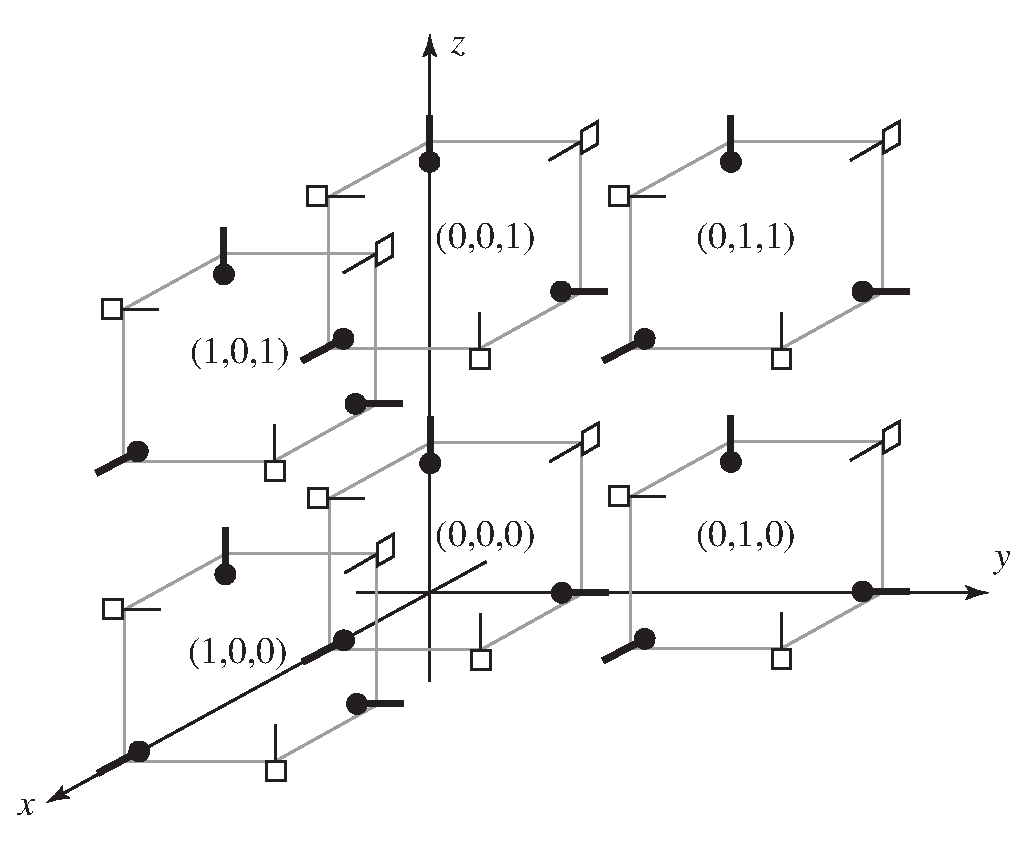
\epsfig{width=4.5in,file=Figures/Fdtd-3d/fdtd-3d-computer.eps}
  \end{center}
  \caption{Arrangement of six groups of nodes where all of the nodes
  within the group have the same set of indices.  The nodes in a group
  are joined by gray lines and their indices are shown as an
  ordered triplet in the center of the group.}  \label{fig:3dComputer}
\end{figure}

In our construction of 3D grids, the faces of the grid will always be
terminated such that there are two electric-field components
tangential to the face and one magnetic field normal to it.  This is
illustrated in Fig.\ \ref{fig:faces3d}.  The computational domain
shown in this figure is one which we describe as having dimensions of
$5\times 9\times 7$ in the $x$, $y$, and $z$ directions, respectively.
Even though we call this a $5\times 9\times 7$ grid, none of the
arrays associated with this computational domain actually have these
dimensions!  The fields of a computational domain that is $M\times
N\times P$ would have dimensions of
\begin{align}
E_x: & \quad (M-1) \times N     \times P   \\
E_y: & \quad M     \times (N-1) \times P   \\
E_z: & \quad M     \times N     \times (P-1) \\
H_x: & \quad M     \times (N-1) \times (P-1) \\
H_y: & \quad (M-1) \times N     \times (P-1) \\
H_z: & \quad (M-1) \times (N-1) \times P
\end{align}
Note that the electric fields have one less element in the direction
in which they point than the nominal size of this grid.  This is
because of the inherent displacement of electric-field nodes in the
direction in which they point.  Rather than having an additional node
essentially sticking beyond the rest of the grid, the array is
truncated in this direction.  Recall that the displacement of the
magnetic-field nodes is in the two directions in which they do not
point.  Thus the magnetic-field arrays are truncated in the two
directions they do not point.  In terms of Yee cubes, an $M\times
N\times P$ grid would consists of $(M-1)\times (N-1)\times (P-1)$
complete cubes.

\begin{figure}
  \begin{center}
  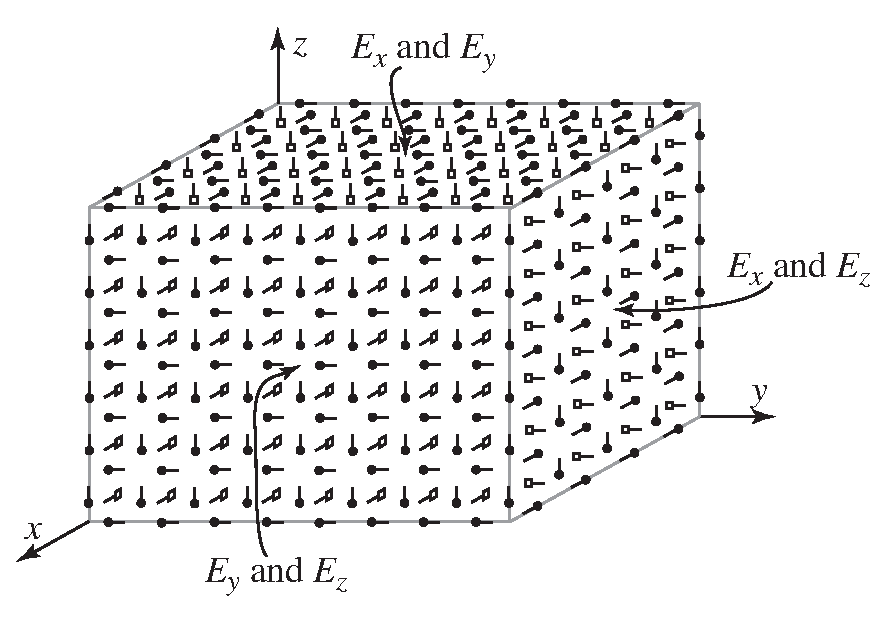
\epsfig{width=5.5in,file=Figures/Fdtd-3d/fdtd-3d-faces.eps}
  \end{center} \caption{Faces of a computational domain which is
  $5\times 9\times 7$ in the $x$, $y$, and $z$ directions,
  respectively.  On the constant-$x$ face the tangential fields are
  $E_y$ and $E_z$, on the constant-$y$ face they are $E_x$ and $E_z$,
  and on the constant-$z$ face they are $E_x$ and $E_y$.  There are also
  magnetic-field nodes which exist on these faces but their orientation
  is normal to the face.}  \label{fig:faces3d}
\end{figure}


\section{3D Example}

Here we provide the code to implement a simple 3D simulation in which
a short dipole source is embedded in a homogeneous domain.  The dipole
is merely an additive source applied to an $E_x$ node in the center of
the grid.  First-order ABC's are used to terminate the grid.  Since
there are two tangential electric fields on each face of the
computational domain, the ABC must be applied to two fields per face.

The {\tt main()} function is shown in Program \ref{pro:3dDemo}.  The
overall structure is little changed from previous simulations.  The
ABC, the grid, the source function, and the snapshot code are
initialized by calling initialization functions outside of the
time-stepping loop.  Within the time-stepping loop the magnetic fields
are updated, the electric fields are updated, the source function is
applied to the $E_x$ node at the center of the grid, the ABC is
applied, and then, assuming it is the appropriate time step, a
snapshot is taken.  Actually, as we will see, two different snapshots
are taken.  There are many ways one might choose to display these 3D
vector fields.  We will merely record one field component over a 2D
plane (or perhaps multiple planes).

\begin{program}
{\tt 3ddemo.c} 3D simulation of an electric dipole realized with an
additive source applied to an $E_x$ node.
\label{pro:3dDemo}
\codemiddle
\begin{lstlisting}
/* 3D simulation with dipole source at center of grid. */

#include "fdtd-alloc.h"
#include "fdtd-macro.h" 
#include "fdtd-proto.h"
#include "ezinc.h"

int main()
{
  Grid *g;

  ALLOC_1D(g, 1, Grid); // allocate memory for grid structure
  gridInit(g);        // initialize 3D grid

  abcInit(g);         // initialize ABC
  ezIncInit(g);
  snapshot3dInit(g);  // initialize snapshots

  /* do time stepping */
  for (Time = 0; Time < MaxTime; Time++) {
    updateH(g);       // update magnetic fields 
    updateE(g);       // update electric fields 
    Ex((SizeX - 1) / 2, SizeY / 2, SizeZ / 2) += ezInc(Time, 0.0);
    abc(g);           // apply ABC
    snapshot3d(g);    // take a snapshot (if appropriate)
  } // end of time-stepping

  return 0;
}
\end{lstlisting}
\end{program}

The code used to realize the source function, i.e., the Ricker
wavelet, is unchanged from before and hence not shown (ref.\ Program
\ref{pro:ricker}).  The header {\tt fdtd-alloc.h} merely provides the
three allocation macros {\tt ALLOC\_1D()}, {\tt ALLOC\_2D()}, and {\tt
  ALLOC\_3D()} and hence is not shown here.  Similarly, the header
{\tt fdtd-grid1.h}, which defines the elements of the {\tt Grid}
structure, is unchanged from before and thus not shown (ref.\ Program
\ref{pro:fdtdgrid1h}).  The header {\tt fdtd-proto.h} provides the
prototypes for the various functions.  Since these prototypes simply
show that each function takes a single argument (i.e., a pointer to a
{\tt Grid} structure), that header file is also not shown.

The header {\tt fdtd-macro.h} shown in Program \ref{pro:fdtdmacro}
provides macros for all the types of grids we have considered so far.
In this particular program we only need the macros for the 3D arrays,
but having created this collection of macros we are well prepared to
use it, unchanged, to tackle a wide variety of FDTD problems.  As was
done in the previous chapter, there are macros which assume that the
{\tt Grid} structure is named {\tt g} while there is another set of
macros that allows the name of the {\tt Grid} to be specified
explicitly.

\begin{program} {\tt fdtd-macro.h} Header that provides the macros to
  access the elements of any of the arrays that have been considered
  thus far.  One set of macros assumes the name of the {\tt Grid} is
  {\tt g}.  Another set allows the name of the {\tt Grid} to be
  specified as an additional argument.
\label{pro:fdtdmacro}
\codemiddle
\begin{lstlisting}
#ifndef _FDTD_MACRO_H
#define _FDTD_MACRO_H

#include "fdtd-grid1.h"

/* macros that permit the "Grid" to be specified */
/* one-dimensional grid */
#define Hy1G(G, M)     G->hy[M]
#define Chyh1G(G, M)   G->chyh[M]
#define Chye1G(G, M)   G->chye[M]

#define Ez1G(G, M)     G->ez[M]
#define Ceze1G(G, M)   G->ceze[M]
#define Cezh1G(G, M)   G->cezh[M]

/* TMz grid */
#define Hx2G(G, M, N)   G->hx[(M) * (SizeYG(G) - 1) + N]
#define Chxh2G(G, M, N) G->chxh[(M) * (SizeYG(G) - 1) + N]
#define Chxe2G(G, M, N) G->chxe[(M) * (SizeYG(G) - 1) + N]

#define Hy2G(G, M, N)   G->hy[(M) * SizeYG(G) + N]
#define Chyh2G(G, M, N) G->chyh[(M) * SizeYG(G) + N]
#define Chye2G(G, M, N) G->chye[(M) * SizeYG(G) + N]

#define Ez2G(G, M, N)   G->ez[(M) * SizeYG(G) + N]
#define Ceze2G(G, M, N) G->ceze[(M) * SizeYG(G) + N]
#define Cezh2G(G, M, N) G->cezh[(M) * SizeYG(G) + N]

/* TEz grid */
#define Ex2G(G, M, N)   G->ex[(M) * SizeYG(G) + N]
#define Cexe2G(G, M, N) G->cexe[(M) * SizeYG(G) + N]
#define Cexh2G(G, M, N) G->cexh[(M) * SizeYG(G) + N]

#define Ey2G(G, M, N)   G->ey[(M) * (SizeYG(G) - 1) + N]
#define Ceye2G(G, M, N) G->ceye[(M) * (SizeYG(G) - 1) + N]
#define Ceyh2G(G, M, N) G->ceyh[(M) * (SizeYG(G) - 1) + N]

#define Hz2G(G, M, N)   G->hz[(M) * (SizeYG(G) - 1) + N]
#define Chzh2G(G, M, N) G->chzh[(M) * (SizeYG(G) - 1) + N]
#define Chze2G(G, M, N) G->chze[(M) * (SizeYG(G) - 1) + N]

/* 3D grid */
#define HxG(G, M, N, P)   G->hx[((M) * (SizeYG(G) - 1) + N) * (SizeZG(G) - 1) + P]
#define ChxhG(G, M, N, P) G->chxh[((M) * (SizeYG(G) - 1) + N) * (SizeZG(G) - 1) + P]
#define ChxeG(G, M, N, P) G->chxe[((M) * (SizeYG(G) - 1) + N) * (SizeZG(G) - 1) + P]

#define HyG(G, M, N, P)   G->hy[((M) * SizeYG(G) + N) * (SizeZG(G) - 1) + P]
#define ChyhG(G, M, N, P) G->chyh[((M) * SizeYG(G) + N) * (SizeZG(G) - 1) + P]
#define ChyeG(G, M, N, P) G->chye[((M) * SizeYG(G) + N) * (SizeZG(G) - 1) + P]

#define HzG(G, M, N, P)   G->hz[((M) * (SizeYG(G) - 1) + N) * SizeZG(G) + P]
#define ChzhG(G, M, N, P) G->chzh[((M) * (SizeYG(G) - 1) + N) * SizeZG(G) + P]
#define ChzeG(G, M, N, P) G->chze[((M) * (SizeYG(G) - 1) + N) * SizeZG(G) + P]

#define ExG(G, M, N, P)   G->ex[((M) * SizeYG(G) + N) * SizeZG(G) + P]
#define CexeG(G, M, N, P) G->cexe[((M) * SizeYG(G) + N) * SizeZG(G) + P]
#define CexhG(G, M, N, P) G->cexh[((M) * SizeYG(G) + N) * SizeZG(G) + P]

#define EyG(G, M, N, P)   G->ey[((M) * (SizeYG(G) - 1) + N) * SizeZG(G) + P]
#define CeyeG(G, M, N, P) G->ceye[((M) * (SizeYG(G) - 1) + N) * SizeZG(G) + P]
#define CeyhG(G, M, N, P) G->ceyh[((M) * (SizeYG(G) - 1) + N) * SizeZG(G) + P]

#define EzG(G, M, N, P)   G->ez[((M) * SizeYG(G) + N) * (SizeZG(G) - 1) + P]
#define CezeG(G, M, N, P) G->ceze[((M) * SizeYG(G) + N) * (SizeZG(G) - 1) + P]
#define CezhG(G, M, N, P) G->cezh[((M) * SizeYG(G) + N) * (SizeZG(G) - 1) + P]

#define SizeXG(G)      G->sizeX
#define SizeYG(G)      G->sizeY
#define SizeZG(G)      G->sizeZ
#define TimeG(G)       G->time
#define MaxTimeG(G)    G->maxTime
#define CdtdsG(G)      G->cdtds
#define TypeG(G)       G->type

/* macros that assume the "Grid" is "g" */
/* one-dimensional grid */
#define Hy1(M)     Hy1G(g, M)
#define Chyh1(M)   Chyh1G(g, M)   
#define Chye1(M)   Chye1G(g, M)   

#define Ez1(M)     Ez1G(g, M)     
#define Ceze1(M)   Ceze1G(g, M)   
#define Cezh1(M)   Cezh1G(g, M)   

/* TMz grid */
#define Hx2(M, N)   Hx2G(g, M, N)   
#define Chxh2(M, N) Chxh2G(g, M, N) 
#define Chxe2(M, N) Chxe2G(g, M, N) 

#define Hy2(M, N)   Hy2G(g, M, N)   
#define Chyh2(M, N) Chyh2G(g, M, N) 
#define Chye2(M, N) Chye2G(g, M, N) 

#define Ez2(M, N)   Ez2G(g, M, N)   
#define Ceze2(M, N) Ceze2G(g, M, N) 
#define Cezh2(M, N) Cezh2G(g, M, N) 

/* TEz grid */
#define Hz2(M, N)   Hz2G(g, M, N)   
#define Chzh2(M, N) Chzh2G(g, M, N) 
#define Chze2(M, N) Chze2G(g, M, N) 

#define Ex2(M, N)   Ex2G(g, M, N)   
#define Cexe2(M, N) Cexe2G(g, M, N) 
#define Cexh2(M, N) Cexh2G(g, M, N) 

#define Ey2(M, N)   Ey2G(g, M, N)   
#define Ceye2(M, N) Ceye2G(g, M, N) 
#define Ceyh2(M, N) Ceyh2G(g, M, N) 

/* 3D grid */
#define Hx(M, N, P)   HxG(g, M, N, P)   
#define Chxh(M, N, P) ChxhG(g, M, N, P) 
#define Chxe(M, N, P) ChxeG(g, M, N, P) 

#define Hy(M, N, P)   HyG(g, M, N, P)   
#define Chyh(M, N, P) ChyhG(g, M, N, P) 
#define Chye(M, N, P) ChyeG(g, M, N, P) 

#define Hz(M, N, P)   HzG(g, M, N, P)   
#define Chzh(M, N, P) ChzhG(g, M, N, P) 
#define Chze(M, N, P) ChzeG(g, M, N, P) 

#define Ex(M, N, P)   ExG(g, M, N, P)   
#define Cexe(M, N, P) CexeG(g, M, N, P) 
#define Cexh(M, N, P) CexhG(g, M, N, P) 

#define Ey(M, N, P)   EyG(g, M, N, P)   
#define Ceye(M, N, P) CeyeG(g, M, N, P) 
#define Ceyh(M, N, P) CeyhG(g, M, N, P) 

#define Ez(M, N, P)   EzG(g, M, N, P)
#define Ceze(M, N, P) CezeG(g, M, N, P)
#define Cezh(M, N, P) CezhG(g, M, N, P) 

#define SizeX       SizeXG(g)
#define SizeY       SizeYG(g)
#define SizeZ       SizeZG(g)
#define Time        TimeG(g)
#define MaxTime     MaxTimeG(g)   
#define Cdtds       CdtdsG(g)
#define Type        TypeG(g)

#endif
\end{lstlisting}
\end{program}

The file {\tt update3d.c} is shown in Program \ref{pro:update3d}.
When {\tt updateE()} or {\tt updateH()} are called they begin by
checking the {\tt Type} of the grid.  These same functions can be
called whether updating a 1D, 2D, or 3D grid.  However, for the 1D
grid there is the assumption that one is dealing with a $z$-polarized
wave and for 2D propagation one has either TM$^z$- or
TE$^z$-polarization.  (A rotation of coordinate systems can be used to
map any 1D simulation to one that is $z$-polarized or any 2D
simulation to one that is either TE$^z$- or TM$^z$-polarized.)

\begin{program}
{\tt update3d.c} Function that can be used to update any of the grids.
\label{pro:update3d}
\codemiddle
\begin{lstlisting}
#include "fdtd-macro.h"
#include <stdio.h>

/* update magnetic field */
void updateH(Grid *g) {
  int mm, nn, pp;

  if (Type == oneDGrid) {
    
    for (mm = 0; mm < SizeX - 1; mm++)
      Hy1(mm) = Chyh1(mm) * Hy1(mm) 
	+ Chye1(mm) * (Ez1(mm + 1) - Ez1(mm));
    
  } else if (Type == tmZGrid) { 
    
    for (mm = 0; mm < SizeX; mm++)
      for (nn = 0; nn < SizeY - 1; nn++)
	Hx2(mm, nn) = Chxh2(mm, nn) * Hx2(mm, nn) 
	  - Chxe2(mm, nn) * (Ez2(mm, nn + 1) - Ez2(mm, nn));
    
    for (mm = 0; mm < SizeX - 1; mm++)
      for (nn = 0; nn < SizeY; nn++)
	Hy2(mm, nn) = Chyh2(mm, nn) * Hy2(mm, nn) 
	  + Chye2(mm, nn) * (Ez2(mm + 1, nn) - Ez2(mm, nn));
    
  } else if (Type == teZGrid) {
    
    for(mm = 0; mm < SizeX - 1; mm++)
      for(nn = 0; nn < SizeY - 1; nn++)
	Hz2(mm, nn) = Chzh2(mm, nn) * Hz2(mm, nn) -
	  Chze2(mm, nn) * ((Ey2(mm + 1, nn) - Ey2(mm, nn)) -
			   (Ex2(mm, nn + 1) - Ex2(mm, nn)));

  } else if (Type == threeDGrid) {
    
    for (mm = 0; mm < SizeX; mm++)
      for (nn = 0; nn < SizeY - 1; nn++)
	for (pp = 0; pp < SizeZ - 1; pp++)
	  Hx(mm, nn, pp) = Chxh(mm, nn, pp) * Hx(mm, nn, pp) +
	    Chxe(mm, nn, pp) * ((Ey(mm, nn, pp + 1) - Ey(mm, nn, pp)) -
				(Ez(mm, nn + 1, pp) - Ez(mm, nn, pp)));
    
    for (mm = 0; mm < SizeX - 1; mm++)
      for (nn = 0; nn < SizeY; nn++)
	for (pp = 0; pp < SizeZ - 1; pp++)
	  Hy(mm, nn, pp) = Chyh(mm, nn, pp) * Hy(mm, nn, pp) +
	    Chye(mm, nn, pp) * ((Ez(mm + 1, nn, pp) - Ez(mm, nn, pp)) -
				(Ex(mm, nn, pp + 1) - Ex(mm, nn, pp)));
    
    for (mm = 0; mm < SizeX - 1; mm++)
      for (nn = 0; nn < SizeY - 1; nn++)
	for (pp = 0; pp < SizeZ; pp++)
	  Hz(mm, nn, pp) = Chzh(mm, nn, pp) * Hz(mm, nn, pp) +
	    Chze(mm, nn, pp) * ((Ex(mm, nn + 1, pp) - Ex(mm, nn, pp)) -
				(Ey(mm + 1, nn, pp) - Ey(mm, nn, pp))); 

  } else {
    fprintf(stderr, "updateH: Unknown grid type.  Terminating...\n");
  }
  
  return;
}  /* end updateH() */


/* update electric field */
void updateE(Grid *g) {
  int mm, nn, pp;
  
  if (Type == oneDGrid) {
    
    for (mm = 1; mm < SizeX - 1; mm++)
      Ez1(mm) = Ceze1(mm) * Ez1(mm) 
	+ Cezh1(mm) * (Hy1(mm) - Hy1(mm - 1));
    
  } else if (Type == tmZGrid) {
    
    for (mm = 1; mm < SizeX - 1; mm++)
      for (nn = 1; nn < SizeY - 1; nn++)
	Ez2(mm, nn) = Ceze2(mm, nn) * Ez2(mm, nn) +
	  Cezh2(mm, nn) * ((Hy2(mm, nn) - Hy2(mm - 1, nn)) -
			   (Hx2(mm, nn) - Hx2(mm, nn - 1)));

  } else if (Type == teZGrid) {
    
    for(mm = 1; mm < SizeX - 1; mm++)
      for(nn = 1; nn < SizeY - 1; nn++)
	Ex2(mm, nn) = Cexe2(mm, nn) * Ex2(mm, nn) +
	  Cexh2(mm, nn) * (Hz2(mm, nn) - Hz2(mm, nn - 1));
    
    for(mm = 1; mm < SizeX - 1; mm++)
      for(nn = 1; nn < SizeY - 1; nn++)
	Ey2(mm, nn) = Ceye2(mm, nn) * Ey2(mm, nn) -
	  Ceyh2(mm, nn) * (Hz2(mm, nn) - Hz2(mm - 1, nn));
    
  } else if (Type == threeDGrid) {
    
    for (mm = 0; mm < SizeX - 1; mm++)
      for (nn = 1; nn < SizeY - 1; nn++)
	for (pp = 1; pp < SizeZ - 1; pp++)
	  Ex(mm, nn, pp) = Cexe(mm, nn, pp) * Ex(mm, nn, pp) +
	    Cexh(mm, nn, pp) * ((Hz(mm, nn, pp) - Hz(mm, nn - 1, pp)) -
				(Hy(mm, nn, pp) - Hy(mm, nn, pp - 1)));
    
    for (mm = 1; mm < SizeX - 1; mm++)
      for (nn = 0; nn < SizeY - 1; nn++)
	for (pp = 1; pp < SizeZ - 1; pp++)
	  Ey(mm, nn, pp) = Ceye(mm, nn, pp) * Ey(mm, nn, pp) + 
	    Ceyh(mm, nn, pp) * ((Hx(mm, nn, pp) - Hx(mm, nn, pp - 1)) -
				(Hz(mm, nn, pp) - Hz(mm - 1, nn, pp)));
    
    for (mm = 1; mm < SizeX - 1; mm++)
      for (nn = 1; nn < SizeY - 1; nn++)
	for (pp = 0; pp < SizeZ - 1; pp++)
	  Ez(mm, nn, pp) = Ceze(mm, nn, pp) * Ez(mm, nn, pp) +
	    Cezh(mm, nn, pp) * ((Hy(mm, nn, pp) - Hy(mm - 1, nn, pp)) -
				(Hx(mm, nn, pp) - Hx(mm, nn - 1, pp)));

  } else {
    fprintf(stderr, "updateE: Unknown grid type.  Terminating...\n");
  }
  
  return;
}  /* end updateE() */
\end{lstlisting}
\end{program}

The code to realize the first-order ABC is shown in Program
\ref{pro:abc3dfirst}.  A first-order ABC requires that a single
``old'' value be recorded for each electric field that is tangential
to a face of the grid.  There are two tangential components per face.
For example, at the ``$x=0$'' face, $E_y$ and $E_z$ are the tangential
components.  These fields are stored in arrays named {\tt Eyx0(n, p)}
and {\tt Ezx0(n, p)}.  The ``{\tt x0}'' part of the name specifies
that these values are at the start of the grid in the $x$-direction.
Since these old fields are recorded over a constant-$x$ face, only the
indices corresponding to the $y$ and $z$ directions are specified
(hence these arrays only take two indices).  The array {\tt Eyx1(n,
  p)} and {\tt Ezx1(n, p)} correspond to the tangential field at the
end of the grid in the $x$-direction.  There are similarly named
arrays for the other two directions.

\begin{program}
{\tt abc3dfirst.c} The code used to implement a first-order ABC on
each face of the 3D domain.
\label{pro:abc3dfirst}
\codemiddle
\begin{lstlisting}
#include "fdtd-alloc.h"
#include "fdtd-macro.h"

/* Macros to access stored "old" value */
#define Eyx0(N, P) eyx0[(N) * (SizeZ) + (P)]
#define Ezx0(N, P) ezx0[(N) * (SizeZ - 1) + (P)]
#define Eyx1(N, P) eyx1[(N) * (SizeZ) + (P)]
#define Ezx1(N, P) ezx1[(N) * (SizeZ - 1) + (P)]

#define Exy0(M, P) exy0[(M) * (SizeZ) + (P)]
#define Ezy0(M, P) ezy0[(M) * (SizeZ - 1) + (P)]
#define Exy1(M, P) exy1[(M) * (SizeZ) + (P)]
#define Ezy1(M, P) ezy1[(M) * (SizeZ - 1) + (P)]

#define Exz0(M, N) exz0[(M) * (SizeY) + (N)]
#define Eyz0(M, N) eyz0[(M) * (SizeY - 1) + (N)]
#define Exz1(M, N) exz1[(M) * (SizeY) + (N)]
#define Eyz1(M, N) eyz1[(M) * (SizeY - 1) + (N)]

/* global variables not visible outside of this package */
static double abccoef = 0.0;
static double *exy0, *exy1, *exz0, *exz1,
  *eyx0, *eyx1, *eyz0, *eyz1,
  *ezx0, *ezx1, *ezy0, *ezy1;

/* initialization function */
void abcInit(Grid *g)
{

  abccoef = (Cdtds - 1.0) / (Cdtds + 1.0);

  /* allocate memory for ABC arrays */
  ALLOC_2D(eyx0, SizeY - 1, SizeZ, double);
  ALLOC_2D(ezx0, SizeY, SizeZ - 1, double);
  ALLOC_2D(eyx1, SizeY - 1, SizeZ, double);
  ALLOC_2D(ezx1, SizeY, SizeZ - 1, double);

  ALLOC_2D(exy0, SizeX - 1, SizeZ, double);
  ALLOC_2D(ezy0, SizeX, SizeZ - 1, double);
  ALLOC_2D(exy1, SizeX - 1, SizeZ, double);
  ALLOC_2D(ezy1, SizeX, SizeZ - 1, double);

  ALLOC_2D(exz0, SizeX - 1, SizeY, double);
  ALLOC_2D(eyz0, SizeX, SizeY - 1, double);
  ALLOC_2D(exz1, SizeX - 1, SizeY, double);
  ALLOC_2D(eyz1, SizeX, SizeY - 1, double);

  return;
}  /* end abcInit() */

/* function that applies ABC -- called once per time step */
void abc(Grid *g)
{
  int mm, nn, pp;
  
  if (abccoef == 0.0) {
    fprintf(stderr,
	    "abc: abcInit must be called before abc.  Terminating...\n");
    exit(-1);
  }

  /* ABC at "x0" */
  mm = 0;
  for (nn = 0; nn < SizeY - 1; nn++)
    for (pp = 0; pp < SizeZ; pp++) {
      Ey(mm, nn, pp) = Eyx0(nn, pp) +
	abccoef * (Ey(mm + 1, nn, pp) - Ey(mm, nn, pp));
      Eyx0(nn, pp) = Ey(mm + 1, nn, pp);
    }
  for (nn = 0; nn < SizeY; nn++)
    for (pp = 0; pp < SizeZ - 1; pp++) {
      Ez(mm, nn, pp) = Ezx0(nn, pp) +
	abccoef * (Ez(mm + 1, nn, pp) - Ez(mm, nn, pp));
      Ezx0(nn, pp) = Ez(mm + 1, nn, pp);
    }
  
  /* ABC at "x1" */
  mm = SizeX - 1;
  for (nn = 0; nn < SizeY - 1; nn++)
    for (pp = 0; pp < SizeZ; pp++) {
      Ey(mm, nn, pp) = Eyx1(nn, pp) +
	abccoef * (Ey(mm - 1, nn, pp) - Ey(mm, nn, pp));
      Eyx1(nn, pp) = Ey(mm - 1, nn, pp);
    }
  for (nn = 0; nn < SizeY; nn++)
    for (pp = 0; pp < SizeZ - 1; pp++) {
      Ez(mm, nn, pp) = Ezx1(nn, pp) +
	abccoef * (Ez(mm - 1, nn, pp) - Ez(mm, nn, pp));
      Ezx1(nn, pp) = Ez(mm - 1, nn, pp);
    }
  
  /* ABC at "y0" */
  nn = 0;
  for (mm = 0; mm < SizeX - 1; mm++)
    for (pp = 0; pp < SizeZ; pp++) {
      Ex(mm, nn, pp) = Exy0(mm, pp) +
	abccoef * (Ex(mm, nn + 1, pp) - Ex(mm, nn, pp));
      Exy0(mm, pp) = Ex(mm, nn + 1, pp);
    }
  for (mm = 0; mm < SizeX; mm++)
    for (pp = 0; pp < SizeZ - 1; pp++) {
      Ez(mm, nn, pp) = Ezy0(mm, pp) +
	abccoef * (Ez(mm, nn + 1, pp) - Ez(mm, nn, pp));
      Ezy0(mm, pp) = Ez(mm, nn + 1, pp);
    }
  
  /* ABC at "y1" */
  nn = SizeY - 1;
  for (mm = 0; mm < SizeX - 1; mm++)
    for (pp = 0; pp < SizeZ; pp++) {
      Ex(mm, nn, pp) = Exy1(mm, pp) +
	abccoef * (Ex(mm, nn - 1, pp) - Ex(mm, nn, pp));
      Exy1(mm, pp) = Ex(mm, nn - 1, pp);
    }
  for (mm = 0; mm < SizeX; mm++)
    for (pp = 0; pp < SizeZ - 1; pp++) {
      Ez(mm, nn, pp) = Ezy1(mm, pp) +
	abccoef * (Ez(mm, nn - 1, pp) - Ez(mm, nn, pp));
      Ezy1(mm, pp) = Ez(mm, nn - 1, pp);
    }
  
  /* ABC at "z0" (bottom) */
  pp = 0;
  for (mm = 0; mm < SizeX - 1; mm++)
    for (nn = 0; nn < SizeY; nn++) {
      Ex(mm, nn, pp) = Exz0(mm, nn) +
	abccoef * (Ex(mm, nn, pp + 1) - Ex(mm, nn, pp));
      Exz0(mm, nn) = Ex(mm, nn, pp + 1);
    }
  for (mm = 0; mm < SizeX; mm++)
    for (nn = 0; nn < SizeY - 1; nn++) {
      Ey(mm, nn, pp) = Eyz0(mm, nn) +
	abccoef * (Ey(mm, nn, pp + 1) - Ey(mm, nn, pp));
      Eyz0(mm, nn) = Ey(mm, nn, pp + 1);
    }
  
  /* ABC at "z1" (top) */
  pp = SizeZ - 1;
  for (mm = 0; mm < SizeX - 1; mm++)
    for (nn = 0; nn < SizeY; nn++) {
      Ex(mm, nn, pp) = Exz1(mm, nn) +
	abccoef * (Ex(mm, nn, pp - 1) - Ex(mm, nn, pp));
      Exz1(mm, nn) = Ex(mm, nn, pp - 1);
    }
  for (mm = 0; mm < SizeX; mm++)
    for (nn = 0; nn < SizeY - 1; nn++) {
      Ey(mm, nn, pp) = Eyz1(mm, nn) +
	abccoef * (Ey(mm, nn, pp - 1) - Ey(mm, nn, pp));
      Eyz1(mm, nn) = Ey(mm, nn, pp - 1);
    }
  
  return;
}  /* end abc() */
\end{lstlisting}
\end{program}

The function to initialize the 3D grid is shown in Program
\ref{pro:grid3dhomo}.  Here the grid is simply homogeneous free space.
The function starts by setting various parameters of the grid, such as
the size and the number of time steps, in lines
\ref{grid3dhomoA}--\ref{grid3dhomoB}.  The function then allocates
space for the various arrays (lines
\ref{grid3dhomoC}--\ref{grid3dhomoD}).  Finally, the function
initializes the values of the coefficient arrays to correspond to free
space (lines \ref{grid3dhomoE}--\ref{grid3dhomoF}).

\begin{program}
{\tt grid3dhomo.c} Function to initialize a homogeneous 3D grid.
\label{pro:grid3dhomo}
\codemiddle
\begin{lstlisting}
#include "fdtd-macro.h"
#include "fdtd-alloc.h"
#include <math.h>

void gridInit(Grid *g) {
  double imp0 = 377.0;
  int mm, nn, pp;

  Type = threeDGrid;   /*@ \label{grid3dhomoA} @*/
  SizeX = 32; // size of domain
  SizeY = 31;
  SizeZ = 31;
  MaxTime = 300; // duration of simulation
  Cdtds = 1.0 / sqrt(3.0); // Courant number /*@ \label{grid3dhomoB} @*/

  /* memory allocation */
  ALLOC_3D(g->hx,   SizeX, SizeY - 1, SizeZ - 1, double); /*@ \label{grid3dhomoC} @*/
  ALLOC_3D(g->chxh, SizeX, SizeY - 1, SizeZ - 1, double);
  ALLOC_3D(g->chxe, SizeX, SizeY - 1, SizeZ - 1, double);
  ALLOC_3D(g->hy,   SizeX - 1, SizeY, SizeZ - 1, double);
  ALLOC_3D(g->chyh, SizeX - 1, SizeY, SizeZ - 1, double);
  ALLOC_3D(g->chye, SizeX - 1, SizeY, SizeZ - 1, double);
  ALLOC_3D(g->hz,   SizeX - 1, SizeY - 1, SizeZ, double);
  ALLOC_3D(g->chzh, SizeX - 1, SizeY - 1, SizeZ, double);
  ALLOC_3D(g->chze, SizeX - 1, SizeY - 1, SizeZ, double);

  ALLOC_3D(g->ex,   SizeX - 1, SizeY, SizeZ, double);
  ALLOC_3D(g->cexe, SizeX - 1, SizeY, SizeZ, double);
  ALLOC_3D(g->cexh, SizeX - 1, SizeY, SizeZ, double);
  ALLOC_3D(g->ey,   SizeX, SizeY - 1, SizeZ, double);
  ALLOC_3D(g->ceye, SizeX, SizeY - 1, SizeZ, double);
  ALLOC_3D(g->ceyh, SizeX, SizeY - 1, SizeZ, double);
  ALLOC_3D(g->ez,   SizeX, SizeY, SizeZ - 1, double);
  ALLOC_3D(g->ceze, SizeX, SizeY, SizeZ - 1, double);
  ALLOC_3D(g->cezh, SizeX, SizeY, SizeZ - 1, double); /*@ \label{grid3dhomoD} @*/
  
  /* set electric-field update coefficients */
  for (mm = 0; mm < SizeX - 1; mm++) /*@ \label{grid3dhomoE} @*/
    for (nn = 0; nn < SizeY; nn++) 
      for (pp = 0; pp < SizeZ; pp++) {
	Cexe(mm, nn, pp) = 1.0;
	Cexh(mm, nn, pp) = Cdtds * imp0;
      }

  for (mm = 0; mm < SizeX; mm++)
    for (nn = 0; nn < SizeY - 1; nn++) 
      for (pp = 0; pp < SizeZ; pp++) {
	Ceye(mm, nn, pp) = 1.0;
	Ceyh(mm, nn, pp) = Cdtds * imp0;
      }

  for (mm = 0; mm < SizeX; mm++)
    for (nn = 0; nn < SizeY; nn++) 
      for (pp = 0; pp < SizeZ - 1; pp++) {
	Ceze(mm, nn, pp) = 1.0;
	Cezh(mm, nn, pp) = Cdtds * imp0;
      }

  /* set magnetic-field update coefficients */
  for (mm = 0; mm < SizeX; mm++)
    for (nn = 0; nn < SizeY - 1; nn++) 
      for (pp = 0; pp < SizeZ - 1; pp++) {
	Chxh(mm, nn, pp) = 1.0;
	Chxe(mm, nn, pp) = Cdtds / imp0;
      }

  for (mm = 0; mm < SizeX - 1; mm++)
    for (nn = 0; nn < SizeY; nn++) 
      for (pp = 0; pp < SizeZ - 1; pp++) {
	Chyh(mm, nn, pp) = 1.0;
	Chye(mm, nn, pp) = Cdtds / imp0;
      }

  for (mm = 0; mm < SizeX - 1; mm++)
    for (nn = 0; nn < SizeY - 1; nn++) 
      for (pp = 0; pp < SizeZ; pp++) {
	Chzh(mm, nn, pp) = 1.0;
	Chze(mm, nn, pp) = Cdtds / imp0;
      } /*@ \label{grid3dhomoF} @*/

  return;
}  /* end gridInit() */
\end{lstlisting}
\end{program}

As mentioned, there are many ways one might display 3D vector data.
Here we merely record the $E_x$ field over a constant-$x$ and a
constant-$y$ plane.  In this way, the core of the snapshot code is
quite similar to that which was used in the 2D simulations.  The
snapshot code to accomplish this is shown in Program
\ref{pro:snapshot3d}.

\begin{program}
{\tt snapshot3d.c}  Functions used to record 2D snapshots of the $E_x$
field.  At the appropriate time steps, two snapshots are taken: one
over a constant-$x$ plane and another over a constant-$y$ plane.
These snapshots are written to separate files.  
\label{pro:snapshot3d}
\codemiddle
\begin{lstlisting}
#include <stdio.h>
#include <stdlib.h>
#include "fdtd-macro.h"

static int temporalStride = -2, frameX = 0, frameY = 0, startTime;
static char basename[80];

void snapshot3dInit(Grid *g) {
  
  int choice;
  
  printf("Do you want 2D snapshots of the 3D grid? (1=yes, 0=no) ");
  scanf("%d", &choice);
  if (choice == 0) {
    temporalStride = -1;
    return;
  }

  printf("Duration of simulation is %d steps.\n", MaxTime);
  printf("Enter start time and temporal stride: ");
  scanf(" %d %d", &startTime, &temporalStride);
  printf("Enter the base name: ");
  scanf(" %s", basename);

  return;
}  /* end snapshot3dInit() */


void snapshot3d(Grid *g) {
  int mm, nn, pp;
  float dim1, dim2, temp;
  char filename[100];
  FILE *out;

  /* ensure temporal stride set to a reasonable value */
  if (temporalStride == -1) {
    return;
  } if (temporalStride < -1) {
    fprintf(stderr,
      "snapshot2d: snapshotInit2d must be called before snapshot.\n"
      "            Temporal stride must be set to positive value.\n");
    exit(-1);
  }

  /* get snapshot if temporal conditions met */
  if (Time >= startTime && 
      (Time - startTime) % temporalStride == 0) {

    /************ write the constant-x slice ************/
    sprintf(filename, "%s-x.%d", basename, frameX++);
    out = fopen(filename, "wb");

    /* write dimensions to output file */
    dim1 = SizeY; // express dimensions as floats
    dim2 = SizeZ; // express dimensions as floats
    fwrite(&dim1, sizeof(float), 1, out);
    fwrite(&dim2, sizeof(float), 1, out);

    /* write remaining data */
    mm = (SizeX - 1) / 2;
    for (pp = SizeZ - 1; pp >= 0; pp--)
      for (nn = 0; nn < SizeY; nn++) {
	temp = (float)Ex(mm, nn, pp); // store data as a float
	fwrite(&temp, sizeof(float), 1, out); // write the float
      }

    fclose(out);  // close file

    /************ write the constant-y slice ************/
    sprintf(filename, "%s-y.%d", basename, frameY++);
    out = fopen(filename, "wb");

    /* write dimensions to output file */
    dim1 = SizeX - 1; // express dimensions as floats
    dim2 = SizeZ; // express dimensions as floats
    fwrite(&dim1, sizeof(float), 1, out);
    fwrite(&dim2, sizeof(float), 1, out);

    /* write remaining data */
    nn = SizeY / 2;
    for (pp = SizeZ - 1; pp >= 0; pp--)
      for (mm = 0; mm < SizeX - 1; mm++) {
	temp = (float)Ex(mm, nn, pp); // store data as a float
	fwrite(&temp, sizeof(float), 1, out); // write the float
      }

    fclose(out);  // close file
  }

  return;
}  /* end snapshot3d() */
\end{lstlisting}
\end{program}

Figure \ref{fig:3dDemoResults} shows snapshots of $E_x$ taken over two
different planes at time step $40$.  The Ricker wavelet is such that
there are $15$ points per wavelength at the most energetic frequency.
The field has been normalized by $0.3$ and three decades of scaling
are used.  In Fig.\ \ref{fig:3dDemoResults}(a), taken over a
constant-$x$ plane, the field is seen to radiate isotropically away
from the dipole source---the dipole is normal to the plane.  In Fig.\
\ref{fig:3dDemoResults}(b), taken over a constant-$y$ plane, the
source is contained in the plane and oriented horizontally.  Therefore
the radiated field is stronger above and below the dipole than along
the line of the dipole.

\begin{figure}
  \begin{center}
  \epsfig{width=3.5in,file=Code/Fdtd-3d/snapshot-x4.eps}
  \\
  (a)
  \\
  \epsfig{width=3.5in,file=Code/Fdtd-3d/snapshot-y4.eps}
  \\
  (b)
  \end{center} 

  \caption{Color map of the $E_x$ field at time-step $40$.  (a) Field
  over a constant-$x$ plane that passes through the source node. (b)
  Field over a constant-$y$ plane that passes through the source
  node.  The field has been normalize by $0.3$ and three decades of
  scaling are used.  These images were generated using the Matlab
  commands in Appendix \ref{ap:render2d}.  The image could be
  interpolated to smooth the obvious pixelization but that is not done
  here in order to emphasizes the inherent discrete nature of the
  simulation.}  \label{fig:3dDemoResults}
\end{figure}

\section{TFSF Boundary}

A total-field scattered-field boundary can be used in 3D grids to
introduce the incident field.  Although we have only considered using
the TFSF boundary to introduce plane waves, it is worth noting that in
principle any field could be introduced over the boundary.  So, for
example, if the incident field were due to a dipole source which was
located physically outside of the grid, the field due to that source
could be introduced over the TFSF boundary.  But, whatever the type of
incident field, one should be careful to ensure that the description of
the incident field over the boundary matches the way the field
actually behaves in the grid.  Simply using the expression for the
incident field in the continuous world will invariably cause some
leakage across the boundary (the amount of leakage can always be
reduced by using a finer discretization and may be acceptably small
for various applications).  Here we will restrict consideration to an
incident plane wave and a one-dimensional auxiliary grid will be used
to determine the incident field.  Furthermore, we will assume the
direction of wave propagation is along one of the grid axes.

Figure \ref{fig:3dTfsfBoundary} shows a 3D computational domain in
which a TFSF boundary exists.  The TFSF boundary can be any shape, but
we will restrict consideration to the cuboid shape shown in the
figure.  The boundary has six faces.  Each face has two electric-field
components and two magnetic-field components tangential to the
boundary.  These are the fields that must have their values corrected
to account for the presence of the TFSF boundary since they will have
at least one neighbor on the opposite side of the boundary.

\begin{figure}
  \begin{center}
  \epsfig{width=4.0in,file=Figures/Fdtd-3d/3d-tfsf.eps}
  \end{center} 
  \caption{Three-dimensional computational domain which contains a
  TFSF boundary.}  \label{fig:3dTfsfBoundary}
\end{figure}

To illustrate the dependence of nodes across the boundary, 2D slices
are taken through a computational domain with nominal dimensions
$9\times 7\times 8$.  Figure \ref{fig:3dTfsfConstantX} shows the
orientation of two constant-$x$ slices.  These slices are separated by
a half spatial-step in the $x$ direction.  The fields contained in
these slices are shown in Fig.\ \ref{fig:3dTfsfSlicesX}.  The TFSF
boundary is shown as a dashed line and nodes that must be corrected
owing to the existence of a neighbor on the other side of the boundary
are enclosed in a ``box'' with rounded edges.  Figure
\ref{fig:3dTfsfSlicesX}(a) shows the plane that contains $E_y$,
$E_z$, and $H_x$ while Fig.\
\ref{fig:3dTfsfSlicesX}(b) contains $E_x$, $H_y$, and $H_z$.
These two slices can be overlain to show the view seen looking along
the $x$ axis.  The TFSF boundary would be specified by the first and
last node associated with the boundary, i.e., two ordered triplets.
The correspondence of these nodes to the boundary dimensions are
indicated by the nodes enclosed by a dashed line and labeled ``First''
and ``Last.''  In the example shown here, the indices of the first
node would be $(2,2,2)$ and the indices of the last node would be
$(6,4,5)$.  (However, from just these two slices we cannot determine
the extent of the TF region in the $x$ direction.  Instead, that will
be shown in subsequent figures.)

\begin{figure}
  \begin{center}
  \epsfig{width=4.0in,file=Figures/Fdtd-3d/3d-tfsf-constant-x.eps}
  \end{center} 
  \caption{Constant-$x$ slices of the computational domain used to
  illustration the relationship of nodes across the TFSF boundary.
  The slices are separated by a half spatial-step in the $x$ direction.}
  \label{fig:3dTfsfConstantX} 
\end{figure}

Note that along the ``bottom'' and ``top'' of the TFSF boundary in
Fig.\ \ref{fig:3dTfsfSlicesX}(a) there are two pairs of nodes that
must be corrected while in Fig.\ \ref{fig:3dTfsfSlicesX}(b) there are
three pairs of nodes that must be corrected.  Similarly, there are
different numbers of pairs along the two sides.  The construction of
the TFSF boundary used here is such that corrections are only applied
to electric fields within the total-field region and are only applied
to magnetic fields in the scattered-field region.

\begin{figure}
  \begin{center}
  \epsfig{width=2.7in,file=Figures/Fdtd-3d/3d-tfsf-slice-x1.eps}\\
  (a)\\
  \vspace{.15in}
  \epsfig{width=2.7in,file=Figures/Fdtd-3d/3d-tfsf-slice-x2.eps}\\
  (b)
  \end{center} 
  \vspace{-.15in}
  \caption{Fields over the constant-$x$ slices depicted in Fig.\
  \ref{fig:3dTfsfConstantX}.  (a) Slice containing $E_y$, $E_z$, and
  $H_x$.  (b) Slice containing $E_x$, $H_y$, and $H_z$.}
  \label{fig:3dTfsfSlicesX} 
\end{figure}

Figure \ref{fig:3dTfsfConstantY} shows the orientation of two
constant-$y$ slices and Fig.\ \ref{fig:3dTfsfSlicesY} shows the fields
over these two slices.  The slices are separated by a half
spatial-step in the $y$ direction.  As before, these slices can be
overlain to see the view looking along the axis (in this case the $y$
axis).  From this view one can see that the first and last indices in
the $x$ direction are $2$ and $6$, respectively.

\begin{figure}
  \begin{center}
  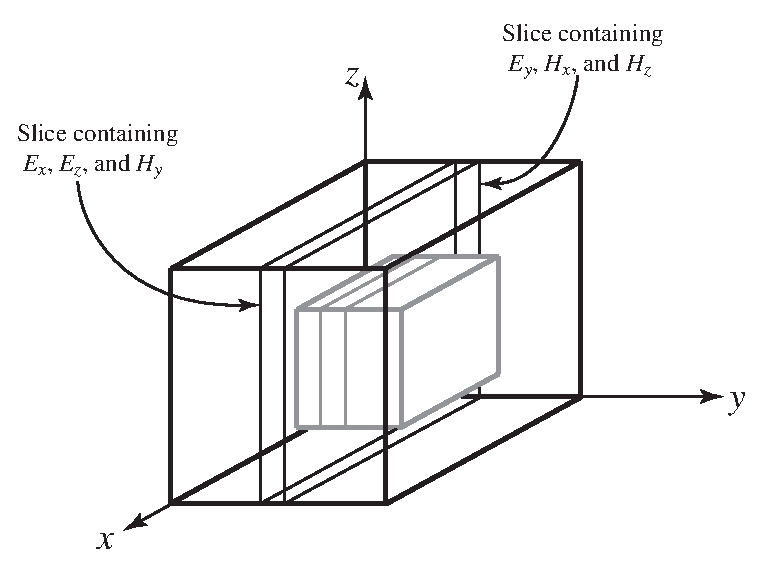
\epsfig{width=4.0in,file=Figures/Fdtd-3d/3d-tfsf-constant-y.eps}
  \end{center} 
  \caption{Constant-$y$ slices of the computational domain used to
  illustration the relationship of nodes across the TFSF boundary.
  The slices are separated by a half spatial-step in the $y$ direction.}
  \label{fig:3dTfsfConstantY}
\end{figure}

\begin{figure}
  \begin{center}
  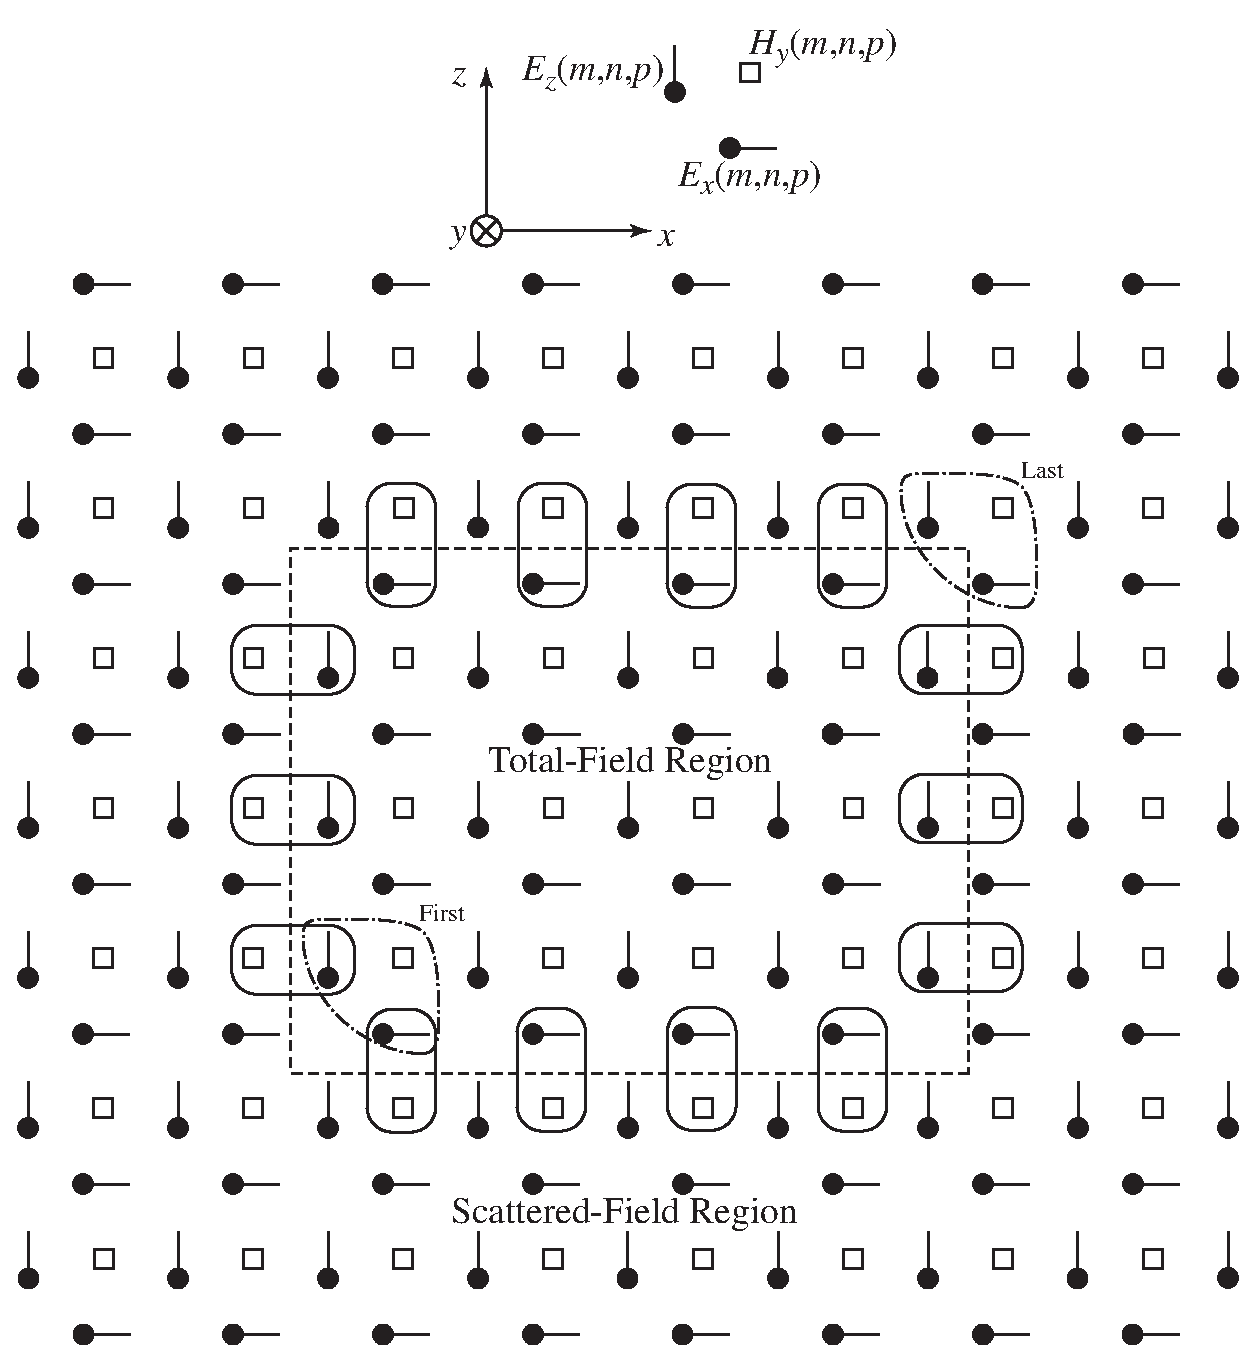
\epsfig{width=3.5in,file=Figures/Fdtd-3d/3d-tfsf-slice-y1.eps}\\
  (a)\\
  \vspace{.15in}
  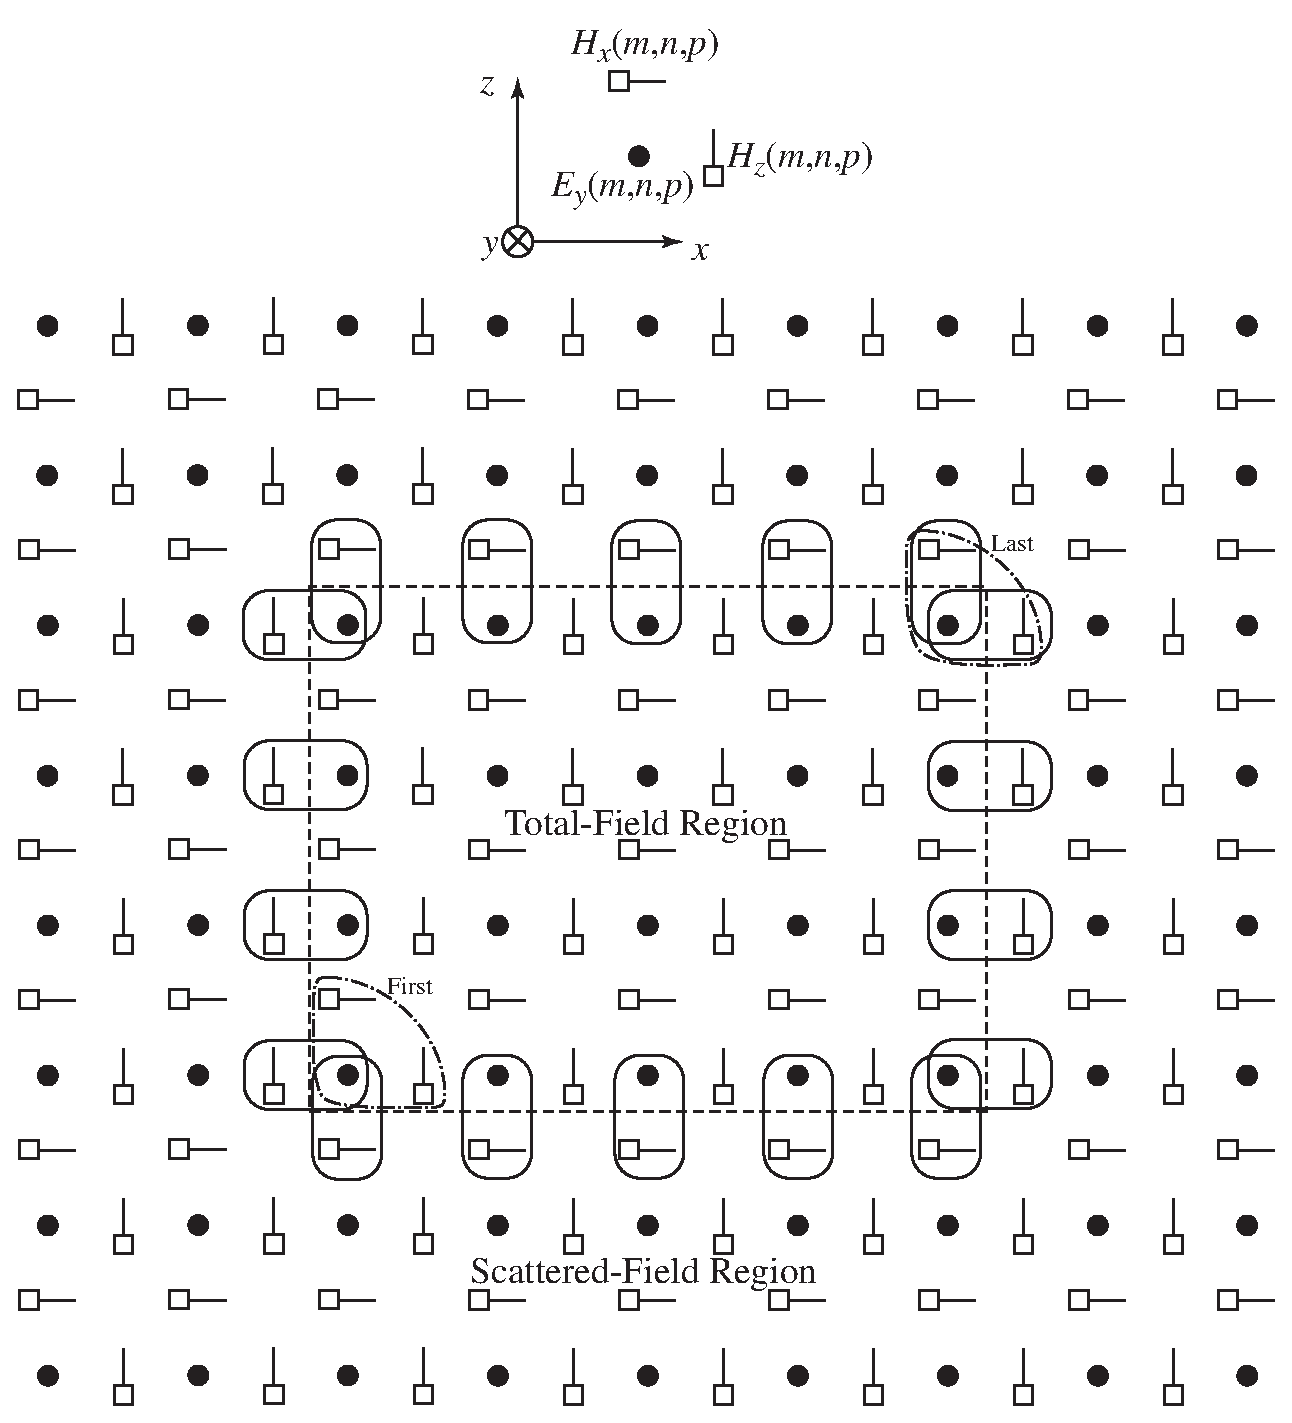
\epsfig{width=3.5in,file=Figures/Fdtd-3d/3d-tfsf-slice-y2.eps}\\
  (b)
  \end{center} 
  \vspace{-.15in}
  \caption{Fields over the constant-$y$ slices depicted in Fig.\
  \ref{fig:3dTfsfConstantY}.  (a) Slice containing $E_x$, $E_z$, and
  $H_y$.  (b) Slice containing $E_y$, $H_x$, and $H_z$.}
  \label{fig:3dTfsfSlicesY} 
\end{figure}

Figure \ref{fig:3dTfsfConstantZ} shows the orientation of two
constant-$z$ slices and Fig.\ \ref{fig:3dTfsfSlicesZ} shows the fields
over these two slices.  The slices are separated by a half
spatial-step in the $z$ direction.  These slices correspond to the
TE$^z$ and TM$^z$ grids which were studied in Chap.\ \ref{chap:multi}.

\begin{figure}
  \begin{center}
  \epsfig{width=4.3in,file=Figures/Fdtd-3d/3d-tfsf-constant-z.eps}
  \end{center} 
  \caption{Constant-$z$ slices of the computational domain used to
  illustration the relationship of nodes across the TFSF boundary.
  The slices are separated by a half spatial-step in the $z$ direction.}
  \label{fig:3dTfsfConstantZ}
\end{figure}

\begin{figure}
  \begin{center}
  \epsfig{width=3.5in,file=Figures/Fdtd-3d/3d-tfsf-slice-z1.eps}\\
  (a)\\
  \vspace{.15in}
  \epsfig{width=3.5in,file=Figures/Fdtd-3d/3d-tfsf-slice-z2.eps}\\
  (b)
  \end{center} 
  \vspace{-.15in}
  \caption{Fields over the constant-$z$ slices depicted in Fig.\
  \ref{fig:3dTfsfConstantZ}.  (a) Slice containing $E_x$, $E_y$, and
  $H_z$.  (b) Slice containing $E_z$, $H_x$, and $H_y$.}
  \label{fig:3dTfsfSlicesZ} 
\end{figure}

Figures \ref{fig:3dTfsfSlicesX}, \ref{fig:3dTfsfSlicesY}, and
\ref{fig:3dTfsfSlicesZ} show all the possible dependencies across the
TFSF boundary.  However, in some applications not all these
dependencies may be relevant.  For example, consider the case when the
incident electric field is polarized in the $z$ direction and
propagating in the $x$ direction.  In this case there are only two
non-zero components of the incident field: $E_z$ and $H_y$.  Thus, not
all of the fields tangential to the TFSF boundary would have to be
corrected.  Only those fields that depend on an $E_z$ or $H_y$ node
on the other side of the boundary would need to be corrected.

Continuing with the assumption of an incident field whose only
non-zero components are $E_z$ and $H_y$, one sees from Fig.\
\ref{fig:3dTfsfSlicesX}(a) that $H_x$ nodes on the constant-$y$ faces
would have to be corrected since they depend on $E_z$ nodes on the
other side of the boundary (these are the nodes along the left and
right side of the TFSF boundary in Fig.\ \ref{fig:3dTfsfSlicesX}(a)).
However, the corresponding $E_z$ nodes would not have to be corrected
because there is no incident $H_x$ field.  From Fig.\
\ref{fig:3dTfsfSlicesX}(b) it is seen that $E_x$ nodes on the
constant-$z$ faces would have to be be corrected since they depend on
$H_y$ on the other side of the boundary.  But, the corresponding $H_y$
nodes do not have to be corrected because there is no incident $E_x$
field.

Figure \ref{fig:3dTfsfSlicesY}(a) shows that $E_x$ must be corrected
over constant-$z$ faces (the top and bottom of the TFSF boundary in
the figure).  (This agrees with the conclusion drawn from inspection
of Fig. \ref{fig:3dTfsfSlicesX}(a).  There is redundant information in
these figures.)  Figure \ref{fig:3dTfsfSlicesY}(a) also shows that
both $E_z$ and $H_y$ must be corrected on constant-$x$ faces.
Inspection of Fig.\ \ref{fig:3dTfsfSlicesY}(b) shows that there is no
need to correct $E_y$, $H_x$, or $H_z$ over constant-$x$ or
constant-$z$ faces since there is no incident field at the nodes that
neighbor these components.

Figure \ref{fig:3dTfsfSlicesZ}(a) indicates, for the assumed incident
field, there is no need to correct $E_x$, $E_y$, or $H_z$ over
constant-$x$ and constant-$y$ faces.  Figure
\ref{fig:3dTfsfSlicesZ}(b) shows that $H_x$ must be corrected over
constant-$y$ faces.  This is the same conclusion one draws from
inspection of Fig.\ \ref{fig:3dTfsfSlicesX}(a). It also shows, as was
seen in Fig.\ \ref{fig:3dTfsfSlicesY}(a), that both $E_z$ and $H_y$
must be corrected over constant-$x$ faces.

\section{TFSF Demonstration}

To demonstrate the implementation of a 3D TFSF boundary, we will model
an incident field that is polarized in the $z$ direction and
propagating in the $x$ direction.  This corresponds to the scenario
described in the previous section.  Because of the given polarization
and direction of propagation, many of the dependencies shown in 
Figs.\ \ref{fig:3dTfsfSlicesX}--\ref{fig:3dTfsfSlicesZ} will not
require any coding.  

The grid will be $35\times 35\times 35$.  A Courant number equal to
the limit of $1/\sqrt{3}$ will be used.  Two simulations will be
performed.  In one there will be no scatterer and in the other a
spherical PEC scatterer will be present.  In 3D, the simplest way to
model a solid PEC is to test if the center of a given Yee cube is
within the PEC.  If it is, as will be shown below, the $12$
electric-field nodes on the edges of the cube are set to zero.

Program \ref{pro:3dTfsfDemo} shows the main body of the program.  This
program is essentially the same as the 2D program that contained a
TFSF boundary (ref.\ Program \ref{pro:tmzdemo2}).  As shown in line
\ref{3dtfsfdemoA}, the TFSF code is initialized by calling an
initialization function outside of the time-stepping loop.  The
corrections to the TFSF boundary are applied by the function {\tt
tfsf()} which, as shown in line
\ref{3dtfsfdemoB}, is called once per time-step.  To work properly,
this function must be called after the magnetic-field update, but
before the electric-field update.  After the magnetic fields are
updated, the function {\tt tfsf()} applies the necessary correction to
the fields tangential to the TFSF boundary.  Immediately after
returning from this function, the electric fields are not in a
consistent state in that the correction has been applied to the
electric fields in anticipation of the impending update.  This is the
same as the case for the 2D implementation of a TFSF boundary
discussed in Sec.\ \ref{sec:tmzTfsf}.

\begin{program}
{\tt 3d-tfsf-demo.c} Main body of a program to implement a TFSF
boundary in 3D.
\label{pro:3dTfsfDemo}
\codemiddle
\begin{lstlisting}
/* 3D simulation with a TFSF boundary. */

#include "fdtd-alloc.h"
#include "fdtd-macro.h" 
#include "fdtd-proto.h"

int main()
{
  Grid *g;

  ALLOC_1D(g, 1, Grid); // allocate memory for grid structure
  gridInit(g);        // initialize 3D grid

  tfsfInit(g);        // initialize TFSF boundary /*@\label{3dtfsfdemoA}@*/
  abcInit(g);         // initialize ABC
  snapshot3dInit(g);  // initialize snapshots

  /* do time stepping */
  for (Time = 0; Time < MaxTime; Time++) {
    updateH(g);     // update magnetic fields 
    tfsf(g);        // apply correction to TFSF boundary /*@\label{3dtfsfdemoB}@*/
    updateE(g);     // update electric fields 
    abc(g);         // apply ABC
    snapshot3d(g);  // take a snapshot (if appropriate)
  } // end of time-stepping

  return 0;
}
\end{lstlisting}
\end{program}

Program \ref{pro:3dTfsfEz} provides the code for the TFSF functions.
The function {\tt tfsfInit()} take a single {\tt Grid} argument, i.e.,
the 3D grid.  There are seven static local variables in this program.
Six of those specify the first and last points in the total-field
region.  The seventh is the {\tt Grid} pointer {\tt g1} that is used
for the 1D auxiliary grid that represents the incident field.  The
initialization function {\tt tfsfInit()} starts by allocating memory
for {\tt g1} and then copying the values from the 3D grid to the 1D
grid.  As discussed in connection with the 2D TFSF boundary, this is
done to ensure the duration and Courant number are the same in both
grids.  Then, in line \ref{tfsf3dezA}, the function {\tt gridInit1D()}
is called to complete the initialization of the 1D grid.  This
function is unchanged from that shown in Program \ref{pro:grid1dez}.
Starting in line \ref{tfsf3dezB}, {\tt tfsfInit()} prompts the user
for indices for the first and last points in the total-field region.
Finally, the source function initialization is called (line
\ref{tfsf3dezD}).  In the results to be shown, the source function was
a Ricker wavelet discretized such that there were $20$ points per
wavelength at the most energetic frequency.

\begin{program}
  {\tt tfsf-3d-ez.c} Three-dimensional TFSF implementation that
  assumes the electric field is polarized in the $z$ direction and
  propagation is in the $x$ direction.
\label{pro:3dTfsfEz}
\codemiddle
\begin{lstlisting}
/* TFSF boundary for a 3D grid.  A 1D auxiliary grid is used to
 * calculate the incident field which is assumed to be propagating in
 * the x direction and polarized in the z direction. */

#include <string.h>  // for memcpy
#include "fdtd-macro.h"
#include "fdtd-proto.h"
#include "fdtd-alloc.h"
#include "ezinc.h"

static int 
    firstX = 0, firstY, firstZ, // indices for first point in TF region
    lastX, lastY, lastZ;        // indices for last point in TF region

static Grid *g1;  // 1D auxiliary grid

void tfsfInit(Grid *g) {

  ALLOC_1D(g1, 1, Grid);       // allocate memory for 1D Grid
  memcpy(g1, g, sizeof(Grid)); // copy information from 3D array
  gridInit1d(g1);              // initialize 1d grid /*@\label{tfsf3dezA}@*/

  printf("Grid is %d by %d by %d.\n", SizeX, SizeY, SizeZ); /*@\label{tfsf3dezB}@*/
  printf("Enter indices for first point in TF region: ");
  scanf(" %d %d %d", &firstX, &firstY, &firstZ);
  printf("Enter indices for last point in TF region: ");
  scanf(" %d %d %d", &lastX, &lastY, &lastZ);

  ezIncInit(g); // initialize source function /*@\label{tfsf3dezD}@*/

  return;
}  /* end tfsfInit() */


void tfsf(Grid *g) {  /*@\label{tfsf3dezC}@*/
  int mm, nn, pp;

  // check if tfsfInit() has been called
  if (firstX <= 0) {
    fprintf(stderr,
      "tfsf: tfsfInit must be called before tfsfUpdate.\n"
      "      Boundary location must be set to positive value.\n");
    exit(-1);
  }

  /****** constant x faces -- scattered-field nodes ******/

  // correct Hy at firstX-1/2 by subtracting Ez_inc
  mm = firstX;
  for (nn = firstY; nn <= lastY; nn++)
    for (pp = firstZ; pp < lastZ; pp++)
      Hy(mm - 1, nn, pp) -= Chye(mm, nn, pp) * Ez1G(g1, mm);

  // correct Hy at lastX + 1/2 by adding Ez_inc
  mm = lastX;
  for (nn = firstY; nn <= lastY; nn++)
    for (pp = firstZ; pp < lastZ; pp++)
      Hy(mm, nn, pp) += Chye(mm, nn, pp) * Ez1G(g1, mm);

  /**** constant y faces -- scattered-field nodes ****/

  // correct Hx at firstY-1/2 by adding Ez_inc
  nn = firstY;
  for (mm = firstX; mm <= lastX; mm++)
    for (pp = firstZ; pp < lastZ; pp++)
      Hx(mm, nn - 1, pp) += Chxe(mm, nn - 1, pp) * Ez1G(g1, mm);

  // correct Hx at lastY+1/2 by subtracting Ez_inc
  nn = lastY;
  for (mm = firstX; mm <= lastX; mm++)
    for (pp = firstZ; pp < lastZ; pp++)
      Hx(mm, nn, pp) -= Chxe(mm, nn, pp) * Ez1G(g1, mm);

  /**** constant z faces -- scattered-field nodes ****/

  // nothing to correct on this face

  /**** update the fields in the auxiliary 1D grid ****/
  updateH(g1);    // update 1D magnetic field
  updateE(g1);    // update 1D electric field
  Ez1G(g1, 0) = ezInc(TimeG(g1), 0.0); // set source node
  TimeG(g1)++;    // increment time in 1D grid

  /**** constant x faces -- total-field nodes ****/

  // correct Ez at firstX face by subtracting Hy_inc
  mm = firstX;
  for (nn = firstY; nn <= lastY; nn++)
    for (pp = firstZ; pp < lastZ; pp++)
      Ez(mm, nn, pp) -= Cezh(mm, nn, pp) * Hy1G(g1, mm - 1);

  // correct Ez at lastX face by adding Hy_inc
  mm = lastX;
  for (nn = firstY; nn <= lastY; nn++)
    for (pp = firstZ; pp < lastZ; pp++)
      Ez(mm, nn, pp) += Cezh(mm, nn, pp) * Hy1G(g1, mm);

  /**** constant y faces -- total-field nodes ****/

  // nothing to correct on this face

  /**** constant z faces -- total-field nodes ****/

  // correct Ex at firstZ face by adding Hy_inc
  pp = firstZ;
  for (mm = firstX; mm < lastX; mm++)
    for (nn = firstY; nn <= lastY; nn++)
      Ex(mm, nn, pp) += Cexh(mm, nn, pp) * Hy1G(g1, mm);

  // correct Ex at lastZ face by subtracting Hy_inc
  pp = lastZ;
  for (mm = firstX; mm < lastX; mm++)
    for (nn = firstY; nn <= lastY; nn++)
      Ex(mm, nn, pp) -= Cexh(mm, nn, pp) * Hy1G(g1, mm);

  return;
}  /* end tfsf() */
\end{lstlisting}
\end{program}

The function {\tt tfsf()} begins on line \ref{tfsf3dezC}.  This
function, which is called once per time-step, applies the corrections
to the various faces of the TFSF boundary as described in the previous
section.

The code to implement the 3D grid is shown in Program
\ref{pro:grid3dsphere}.  This code is almost identical to the code for
the homogeneous grid that was given in Program \ref{pro:grid3dhomo}.
The the only significant difference is the possible inclusion of the
PEC sphere.  The variables associated with the sphere are listed in
lines \ref{grid3dsphereA} and \ref{grid3dsphereB}.  The users is
queried if the sphere is present.  If it is, the variable {\tt
  isSpherePresent} is set to one.  Otherwise it is set to zero.  The
radius of the sphere, which is stored in {\tt radius}, is set to $8$
cells while the indices for the center of the sphere are set to
$(17,17,17)$.  The grid is initially set to uniform free space.
However, if the sphere is present, as shown starting at line
\ref{grid3dsphereC}, the center of each Yee cube is checked.  If it is
within a distance of {\tt radius} cells from the center of the sphere,
all $12$ electric-field nodes on the edges of the cube are set to
zero.  (In the for-loops associated with this check, the squared
values of the distances are used so as to avoid having to calculate
square roots.)  The update coefficients for the magnetic field are
unaffected by the presence of the PEC.

\begin{program}
  {\tt grid3dsphere.c} Function to initialize a {\tt Grid} structure.
  The user is prompted to determine if a PEC sphere of radius 8-cells
  should be present.  If it is not, the grid is homogeneous free
  space.
\label{pro:grid3dsphere}
\codemiddle
\begin{lstlisting}
#include "fdtd-macro.h"
#include "fdtd-alloc.h"
#include <math.h>

void gridInit(Grid *g) {
  double imp0 = 377.0;
  int mm, nn, pp;

  // sphere parameters
  int m_c = 17, n_c = 17, p_c = 17, isSpherePresent; /*@\label{grid3dsphereA}@*/
  double m2, n2, p2, r2, radius = 8.0;              /*@\label{grid3dsphereB}@*/

  Type    = threeDGrid;
  SizeX   = 35; // size of domain
  SizeY   = 35;
  SizeZ   = 35;
  MaxTime = 300; // duration of simulation
  Cdtds   = 1.0 / sqrt(3.0); // Courant number

  printf("If the sphere present: (1=yes, 0=no) ");
  scanf(" %d", &isSpherePresent);

  /* memory allocation */
  ALLOC_3D(g->hx,   SizeX, SizeY - 1, SizeZ - 1, double);
  ALLOC_3D(g->chxh, SizeX, SizeY - 1, SizeZ - 1, double);
  ALLOC_3D(g->chxe, SizeX, SizeY - 1, SizeZ - 1, double);
  ALLOC_3D(g->hy,   SizeX - 1, SizeY, SizeZ - 1, double);
  ALLOC_3D(g->chyh, SizeX - 1, SizeY, SizeZ - 1, double);
  ALLOC_3D(g->chye, SizeX - 1, SizeY, SizeZ - 1, double);
  ALLOC_3D(g->hz,   SizeX - 1, SizeY - 1, SizeZ, double);
  ALLOC_3D(g->chzh, SizeX - 1, SizeY - 1, SizeZ, double);
  ALLOC_3D(g->chze, SizeX - 1, SizeY - 1, SizeZ, double);

  ALLOC_3D(g->ex,   SizeX - 1, SizeY, SizeZ, double);
  ALLOC_3D(g->cexe, SizeX - 1, SizeY, SizeZ, double);
  ALLOC_3D(g->cexh, SizeX - 1, SizeY, SizeZ, double);
  ALLOC_3D(g->ey,   SizeX, SizeY - 1, SizeZ, double);
  ALLOC_3D(g->ceye, SizeX, SizeY - 1, SizeZ, double);
  ALLOC_3D(g->ceyh, SizeX, SizeY - 1, SizeZ, double);
  ALLOC_3D(g->ez,   SizeX, SizeY, SizeZ - 1, double);
  ALLOC_3D(g->ceze, SizeX, SizeY, SizeZ - 1, double);
  ALLOC_3D(g->cezh, SizeX, SizeY, SizeZ - 1, double);
  
  /* set electric-field update coefficients */
  for (mm = 0; mm < SizeX - 1; mm++)
    for (nn = 0; nn < SizeY; nn++) 
      for (pp = 0; pp < SizeZ; pp++) {
	Cexe(mm, nn, pp) = 1.0;
	Cexh(mm, nn, pp) = Cdtds * imp0;
      }

  for (mm = 0; mm < SizeX; mm++)
    for (nn = 0; nn < SizeY - 1; nn++) 
      for (pp = 0; pp < SizeZ; pp++) {
	Ceye(mm, nn, pp) = 1.0;
	Ceyh(mm, nn, pp) = Cdtds * imp0;
      }

  for (mm = 0; mm < SizeX; mm++)
    for (nn = 0; nn < SizeY; nn++) 
      for (pp = 0; pp < SizeZ - 1; pp++) {
	Ceze(mm, nn, pp) = 1.0;
	Cezh(mm, nn, pp) = Cdtds * imp0;
      }

  // zero the nodes associated with the PEC sphere
  if (isSpherePresent) { /*@\label{grid3dsphereC}@*/
    r2 = radius * radius;
    for (mm = 2; mm < SizeX - 2; mm++) {
      m2 = (mm + 0.5 - m_c) * (mm + 0.5 - m_c);
      for (nn = 2; nn < SizeY - 2; nn++) {
	n2 = (nn + 0.5 - n_c) * (nn + 0.5 - n_c);
	for (pp = 2; pp < SizeZ - 2; pp++) {
	  p2 = (pp + 0.5 - p_c) * (pp + 0.5 - p_c);
	  // if distance to center of a cube is less than radius 
	  // of the sphere, zero all the surrounding electric
	  // field nodes
	  if (m2 + n2 + p2 < r2) {
	    // zero surrounding Ex nodes
	    Cexe(mm, nn,  pp) = 0.0;
	    Cexe(mm, nn + 1, pp) = 0.0;
	    Cexe(mm, nn,  pp + 1) = 0.0;
	    Cexe(mm, nn + 1, pp + 1) = 0.0;
	    Cexh(mm, nn,  pp) = 0.0;
	    Cexh(mm, nn + 1, pp) = 0.0;
	    Cexh(mm, nn,  pp + 1) = 0.0;
	    Cexh(mm, nn + 1, pp + 1) = 0.0;
	    // zero surrounding Ey nodes
	    Ceye(mm, nn, pp) = 0.0;
	    Ceye(mm + 1, nn, pp) = 0.0;
	    Ceye(mm, nn, pp + 1) = 0.0;
	    Ceye(mm + 1, nn, pp + 1) = 0.0;
	    Ceyh(mm, nn, pp) = 0.0;
	    Ceyh(mm + 1, nn, pp) = 0.0;
	    Ceyh(mm, nn, pp + 1) = 0.0;
	    Ceyh(mm + 1, nn, pp + 1) = 0.0;
	    // zero surrounding Ez nodes
	    Ceze(mm, nn, pp) = 0.0;
	    Ceze(mm + 1, nn, pp) = 0.0;
	    Ceze(mm, nn + 1, pp) = 0.0;
	    Ceze(mm + 1, nn + 1, pp) = 0.0;
	    Cezh(mm, nn,  pp) = 0.0;
	    Cezh(mm + 1, nn,  pp) = 0.0;
	    Cezh(mm, nn + 1, pp) = 0.0;
	    Cezh(mm + 1, nn + 1, pp) = 0.0;
	  }
	}
      }
    }
  }


  /* set magnetic-field update coefficients */
  for (mm = 0; mm < SizeX; mm++)
    for (nn = 0; nn < SizeY - 1; nn++) 
      for (pp = 0; pp < SizeZ - 1; pp++) {
	Chxh(mm, nn, pp) = 1.0;
	Chxe(mm, nn, pp) = Cdtds / imp0;
      }

  for (mm = 0; mm < SizeX - 1; mm++)
    for (nn = 0; nn < SizeY; nn++) 
      for (pp = 0; pp < SizeZ - 1; pp++) {
	Chyh(mm, nn, pp) = 1.0;
	Chye(mm, nn, pp) = Cdtds / imp0;
      }

  for (mm = 0; mm < SizeX - 1; mm++)
    for (nn = 0; nn < SizeY - 1; nn++) 
      for (pp = 0; pp < SizeZ; pp++) {
	Chzh(mm, nn, pp) = 1.0;
	Chze(mm, nn, pp) = Cdtds / imp0;
      }

  return;
}  /* end gridInit() */
\end{lstlisting}
\end{program}

Figure \ref{fig:3dTfsfDemo} show the $E_z$ field take over a constant
$y$ slice along the center of the computational domain.  The figures on
the left show the field when there is no scatterer while the figures
on the right show the field at the same time-step but when the
spherical scatterer is present.  In the absence of a scatterer, one
can see that there are no fields in the scattered-field region.  The
first point in the total-field region has indices of $(5,5,5)$ while
the last point had indices of $(30,30,30)$.

\begin{figure}
  \begin{center}
  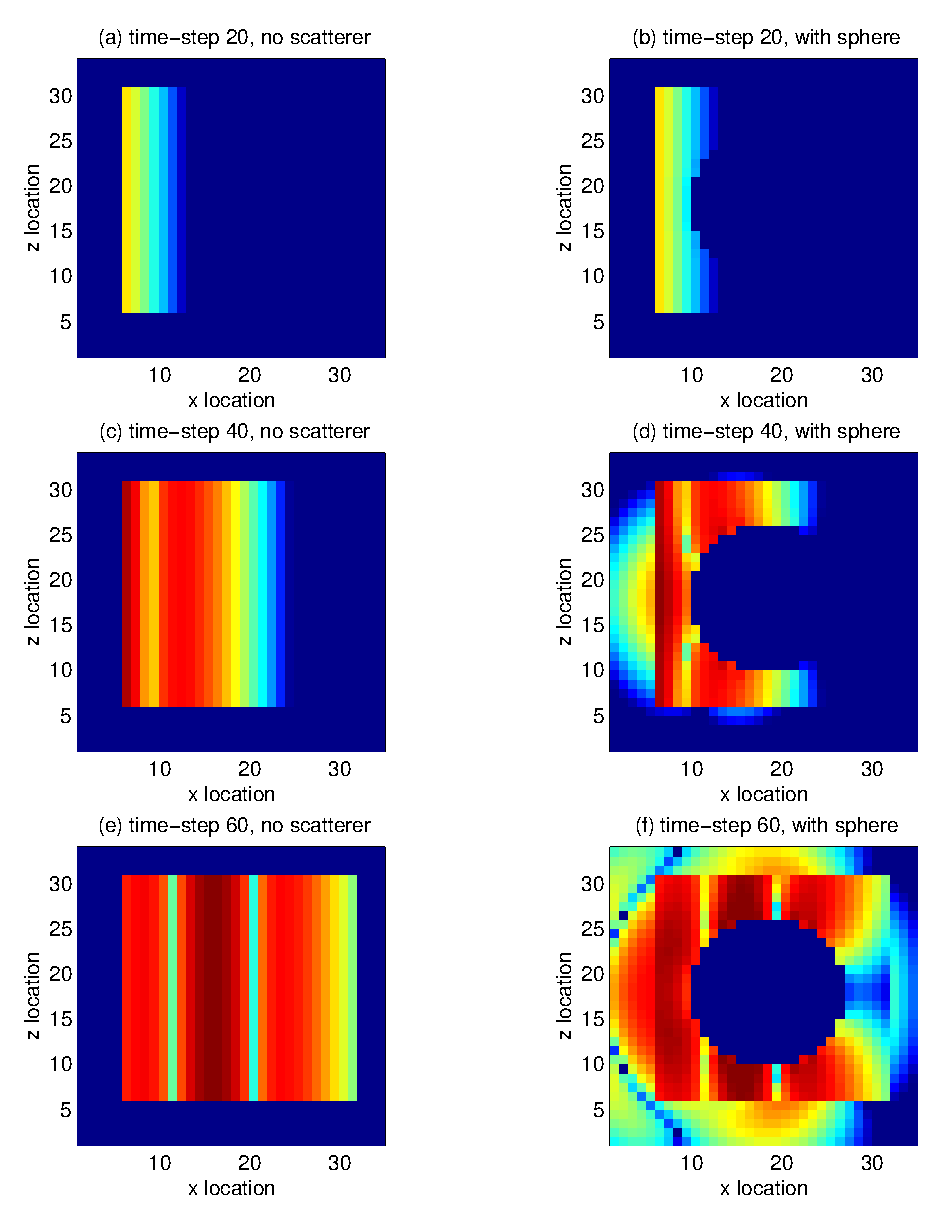
\epsfig{width=6.in,file=Code/Fdtd-3d/Tfsf-new/tfsf-demo.eps}
  \end{center} 
  \caption{The $E_z$ field over a constant-$y$ plane taken from a 3D
    simulation in which the incident electric field is $z$-polarized
    and propagation is in the $x$ direction.  In the figures on the
    left no scatterer is present.  Figures (a), (c), and (e) are taken
    at time-steps, 20, 40, and 60, respectively.  The figures on the
    right show the field at the same time-steps, but a spherical
    scatterer is present.}
  \label{fig:3dTfsfDemo} 
\end{figure}

In these simulations a first-order ABC is used and the code is
unchanged from that presented in Program \ref{pro:abc3dfirst}.  The
snapshot code used to generate the data for Fig.\ \ref{fig:3dTfsfDemo}
is slightly different from Program \ref{pro:snapshot3d} in that here
the $E_z$ field is being recorded while in Program
\ref{pro:snapshot3d} the $E_x$ field was being recorded.  However,
this represents a minor change and hence the modified snapshot code is
not shown.  Another minor change that is not explicitly shown is that
it would be necessary for the header file {\tt fdtd-proto.h} to
include the prototypes for the TFSF functions {\tt tfsfInit()} and
{\tt tfsf()}.  As with nearly all the other functions, these
prototypes would merely show that these functions have a pointer to a
{\tt Grid} structure as their single argument.

\section{Unequal Spatial Steps}

In the previous discussion we have always assumed that
$\Delx=\Dely=\Delz=\delta$.  But how do things change if
$\Delx\neq\Dely\neq\Delz$?  We will consider that question in this
section.  First, let us introduce the following notation
\begin{align*}
\delta  =  \Delx &\quad \Rightarrow \quad \Delx = \delta,\\
r_y     =  \frac{\Dely}{\Delx} &\quad \Rightarrow \quad \Dely = r_y \delta,\\
r_z     =  \frac{\Delz}{\Delx} &\quad \Rightarrow \quad \Delz = r_z \delta.
\end{align*}
Furthermore, we will defined scaled field quantities such that
\begin{eqnarray*}
e_x & = & \Delx E_x, \qquad\qquad h_x  =  \Delx H_x, \\
e_y & = & \Dely E_y, \qquad\qquad h_y  =  \Dely H_y, \\
e_z & = & \Delz E_z, \qquad\qquad h_z  =  \Delz H_z.
\end{eqnarray*}
With these definitions in place, let us consider a rewritten form of
\refeq{eq:exThreeDUpdate}
\begin{multline}
  \frac{1}{\Delx}\fdtdh{\Delx E_x}{m+\half,n,p}{q+1} =
   \frac{1-\frac{\sigma\Delt}{2\epsilon}}{1+\frac{\sigma\Delt}{2\epsilon}}
   \frac{1}{\Delx}\fdtdh{\Delx E_x}{m+\half,n,p}{q} \\
   \hspace{.08in}\mbox{} +
   \frac{1}{1+\frac{\sigma\Delt}{2\epsilon}}
    \left(
    \frac{\Delt}{\epsilon\Dely\Delz}
    \left\{\fdtdh{\Delz H_z}{m+\half,n+\half,p}{q+\half}-
           \fdtdh{\Delz H_z}{m+\half,n-\half,p}{q+\half}\right\}\right.
   \\
    \left. \mbox{} -
    \frac{\Delt}{\epsilon\Dely\Delz}
    \left\{\fdtdh{\Dely H_y}{m+\half,n,p+\half}{q+\half}-
           \fdtdh{\Dely H_y}{m+\half,n,p-\half}{q+\half}\right\}\right).
\end{multline}
Multiplying through by $\Delx$ and employing the definitions given
above, this update equation becomes
\begin{multline}
  \fdtdh{e_x}{m+\half,n,p}{q+1} =
   \frac{1-\frac{\sigma\Delt}{2\epsilon}}{1+\frac{\sigma\Delt}{2\epsilon}}
   \fdtdh{e_x}{m+\half,n,p}{q} \\
   \hspace{.08in}\mbox{} +
   \frac{1}{1+\frac{\sigma\Delt}{2\epsilon}}
    \frac{\Delt}{\epsilon\delta}\frac{1}{r_yr_z}
    \left(
    \left\{\fdtdh{h_z}{m+\half,n+\half,p}{q+\half}-
           \fdtdh{h_z}{m+\half,n-\half,p}{q+\half}\right\}\right.
   \\
    \left. \mbox{} -
    \left\{\fdtdh{h_y}{m+\half,n,p+\half}{q+\half}-
           \fdtdh{h_y}{m+\half,n,p-\half}{q+\half}\right\}\right).
\end{multline}
Importantly, all the (scaled) magnetic fields are multiplied by the
same coefficient.  

From inspection of \refeq{eq:exThreeDUpdate}, it might have appeared
that when the spatial step sizes are not equal, another set of
coefficients would have to be introduced (i.e., one for the term
involving $1/\Dely$ and one for the term involving $1/\Delz$).  This
is true if the field components are not scaled by their respective
lengths.  However, by scaling the fields, it is still only necessary
to have two coefficients per update equation.

The complete set up update equations for the scaled fields are:
\begin{multline}
  \fdtdh{h_x}{m,n+\half,p+\half}{q+\half} =
  \frac{1-\frac{\sigma_m\Delt}{2\mu}}{1+\frac{\sigma_m\Delt}{2\mu}}
  \fdtdh{h_x}{m,n+\half,p+\half}{q-\half} \\
  \hspace{.68in}\mbox{} +
  \frac{1}{1+\frac{\sigma_m\Delt}{2\mu}}
  \frac{\Delt}{\mu\delta}\frac{1}{r_y r_z}
  \left(
    \left\{
      \fdtdh{e_y}{m,n+\half,p+1}{q} -
      \fdtdh{e_y}{m,n+\half,p}{q}
     \right\}
  \right. \\
  \left. \mbox{} -
    \left\{
      \fdtdh{e_z}{m,n+1,p+\half}{q} -
      \fdtdh{e_z}{m,n,p+\half}{q}
    \right\}
  \right),
\end{multline}
\begin{multline}
  \fdtdh{h_y}{m+\half,n,p+\half}{q+\half} =
  \frac{1-\frac{\sigma_m\Delt}{2\mu}}{1+\frac{\sigma_m\Delt}{2\mu}}
  \fdtdh{h_y}{m+\half,n,p+\half}{q-\half} \\
  \hspace{.68in}\mbox{} + 
  \frac{1}{1+\frac{\sigma_m\Delt}{2\mu}}
  \frac{\Delt}{\mu\delta}\frac{r_y}{r_z}
  \left(
    \left\{
      \fdtdh{e_z}{m+1,n,p+\half}{q} -
      \fdtdh{e_z}{m,n,p+\half}{q}
    \right\}
  \right.\\
  \left.\mbox{} -
    \left\{
      \fdtdh{e_x}{m+\half,n,p+1}{q} -
      \fdtdh{e_x}{m+\half,n,p}{q}
    \right\}
  \right),
\end{multline}
\begin{multline}
  \lefteqn{\fdtdh{h_z}{m+\half,n+\half,p}{q+\half} =
  \frac{1-\frac{\sigma_m\Delt}{2\mu}}{1+\frac{\sigma_m\Delt}{2\mu}}
  \fdtdh{h_z}{m+\half,n+\half,p}{q-\half}}
  \\
  \hspace{.68in}\mbox{} +
  \frac{1}{1+\frac{\sigma_m\Delt}{2\epsilon}}
  \frac{\Delt}{\mu\delta}\frac{r_z}{r_y}
  \left(
    \left\{
      \fdtdh{e_x}{m+\half,n+1,p}{q} - 
      \fdtdh{e_x}{m+\half,n,p}{q}
    \right\} 
  \right. \\
  \left. \mbox{} -
    \left\{
      \fdtdh{e_y}{m+1,n+\half,p}{q} - 
      \fdtdh{e_y}{m,n+\half,p}{q}
    \right\}
  \right).
\end{multline}
\begin{multline}
  \fdtdh{e_x}{m+\half,n,p}{q+1} =
   \frac{1-\frac{\sigma\Delt}{2\epsilon}}{1+\frac{\sigma\Delt}{2\epsilon}}
   \fdtdh{e_x}{m+\half,n,p}{q} \\
   \hspace{.08in}\mbox{} +
   \frac{1}{1+\frac{\sigma\Delt}{2\epsilon}}
   \frac{\Delt}{\epsilon\delta}\frac{1}{r_yr_z}
   \left(
     \left\{
       \fdtdh{h_z}{m+\half,n+\half,p}{q+\half} -
       \fdtdh{h_z}{m+\half,n-\half,p}{q+\half}
     \right\}
   \right. \\
   \left. \mbox{} -
     \left\{
       \fdtdh{h_y}{m+\half,n,p+\half}{q+\half} -
       \fdtdh{h_y}{m+\half,n,p-\half}{q+\half}
     \right\}
   \right).
\end{multline}
\begin{multline}
  \fdtdh{e_y}{m,n+\half,p}{q+1} =
   \frac{1-\frac{\sigma\Delt}{2\epsilon}}{1+\frac{\sigma\Delt}{2\epsilon}}
   \fdtdh{e_y}{m,n+\half}{q} \\
   \hspace{.08in}\mbox{} +
   \frac{1}{1+\frac{\sigma\Delt}{2\epsilon}}
   \frac{\Delt}{\epsilon\delta}\frac{r_y}{r_z}
   \left(
     \left\{
       \fdtdh{h_x}{m,n+\half,p-\half}{q+\half} -
       \fdtdh{h_x}{m,n+\half,p-\half}{q+\half}
     \right\}
   \right. \\
   \left. \mbox{} -
     \left\{
       \fdtdh{h_z}{m+\half,n+\half,p}{q+\half} -
       \fdtdh{h_z}{m-\half,n+\half,p}{q+\half}
     \right\}
   \right),
\end{multline}
\begin{multline}
  \lefteqn{\fdtdh{e_z}{m,n,p+\half}{q+1} =
  \frac{1-\frac{\sigma\Delt}{2\epsilon}}{1+\frac{\sigma\Delt}{2\epsilon}}
  \fdtdh{e_z}{m,n,p+\half}{q}} \\
  \hspace{.08in}\mbox{} +
  \frac{1}{1+\frac{\sigma\Delt}{2\epsilon}}
  \frac{\Delt}{\epsilon\delta}\frac{r_z}{r_y}
  \left(
    \left\{
      \fdtdh{h_y}{m+\half,n,p+\half}{q+\half} -
      \fdtdh{h_y}{m-\half,n,p+\half}{q+\half}
    \right\}
  \right. \\
  \left. \mbox{} - 
    \left\{
      \fdtdh{h_x}{m,n+\half,p+\half}{q+\half} -
      \fdtdh{h_x}{m,n-\half,p+\half}{q+\half}
    \right\}
  \right).
\end{multline}

Thinking now in terms of coefficients, note that all the ``self-term''
coefficients are virtually unchanged from those given previously,
i.e., $\chxh$, $\chyh$, $\chzh$, $\cexe$, $\ceye$, and $\ceze$ are as
given in \refeq{eq:chxhDef}, \refeq{eq:chyhDef}, \refeq{eq:chzhDef},
\refeq{eq:cexeDef}, \refeq{eq:ceyeDef}, and \refeq{eq:cexeDef},
respectively.  (There is a slight difference in that those expressions
listed the evaluation points merely in terms of a uniform spatial step
size of $\delta$---one would now have to think in terms of $\Delx$,
$\Dely$, and $\Delz$, for displacements in the $x$, $y$, and $z$
directions, respectively.)

The ``cross'' coefficients, such as $\chze$ and $\ceyh$, are nearly
the same as before where the only differences are that $\delta$
specifically represents the spatial step $\Delx$, the scale factors
$r_y$ and $r_z$ now appear, and the locations are specifically in
terms of $\Delx$, $\Dely$, and $\Delz$.  These scaled coefficients are
now
\begin{align}
\chxe(m,n+1/2,p+1/2) &=
  \left.
  \frac{1}{1+\frac{\sigma_m\Delt}{2\mu}}
  \frac{\Delt}{\mu\delta} \frac{1}{r_y r_z}
  \right|_{m\Delx,(n+1/2)\Dely,(p+1/2)\Delz}, 
  \label{eq:chxeScaled} \\
\chye(m+1/2,n,p+1/2) &=
  \left.
  \frac{1}{1+\frac{\sigma_m\Delt}{2\mu}}
  \frac{\Delt}{\mu\delta} \frac{r_y}{r_z}
  \right|_{(m+1/2)\Delx,n\Dely,(p+1/2)\Delz}, \\
\chze(m+1/2,n+1/2,p) &=
  \left.
  \frac{1}{1+\frac{\sigma_m\Delt}{2\mu}}
  \frac{\Delt}{\mu\delta} \frac{r_z}{r_y}
  \right|_{(m+1/2)\Delx,(n+1/2)\Dely,p\Delz}, \\
\cexh(m+1/2,n,p) &=
  \left.
  \frac{1}{1+\frac{\sigma\Delt}{2\epsilon}}
  \frac{\Delt}{\epsilon\delta} \frac{1}{r_y r_z}
  \right|_{(m+1/2)\Delx,n\Dely,p\Delz}, \\
\ceyh(m,n+1/2,p) &= 
  \left.
  \frac{1}{1+\frac{\sigma\Delt}{2\epsilon}}
    \frac{\Delt}{\epsilon\delta} \frac{r_y}{r_z}
  \right|_{m\Delx,(n+1/2)\Dely,p\Delz}, \\
\cezh(m,n,p+1/2) &=
  \left.
  \frac{1}{1+\frac{\sigma\Delt}{2\epsilon}}
    \frac{\Delt}{\epsilon\delta} \frac{r_z}{r_y}
  \right|_{m\Delx,n\Dely,(p+1/2)\Delz}.
  \label{eq:cezhScaled}
\end{align}

Finally, stability dictates that 
\begin{equation}
\Delt \leq 
  \frac{1}{c\sqrt{\frac{1}{\Delx^2} +
                  \frac{1}{\Dely^2} +
                  \frac{1}{\Delz^2}}}
\end{equation}
which, after employing the definitions given above and rearranging,
can be written as
\begin{equation}
\frac{c\Delt}{\delta} \leq 
  \frac{1}{\sqrt{1 + \frac{1}{r_y^2} + \frac{1}{r_z^2}}}
  \label{eq:courantUnequalSpace}
\end{equation}

Note that when $r_y=r_z=1$ all the update equations and coefficients
are identical to what was previously given for a uniform grid.  This
may seem rather odd because now we are discussing scaled fields
instead of the fields themselves, e.g., we are dealing with $e_x=\Delx
E_x$ instead of $E_x$.  (The scaled ``electric'' and ``magnetic''
fields have units of volts and amperes, respectively, instead of volts
per meter and ampere per meter, and hence these fields are really
voltages and currents.)  However, one must keep in mind that for these
scaled fields the source terms would corresponding have to be scaled.
For example, if there were an additive source current in the update
equation for $E_x$, in the scaled version of the update equation this
source term would also be scaled by $\Delx$.  Thus, if one were to
compare the values in a simulation involving the scaled and unscaled
$x$-component of the electric field, the scaled values would be larger
by a factor of $\Delx$.  When the scaled field is divided by $\Delx$
one obtains the same electric field that would be obtained directly
from a simulation with unscaled fields.

Returning to the question raised at the beginning of the section: But
how do things change if $\Delx\neq\Dely\neq\Delz$?  The answer is that
very little changes.  The same code can be used for simulations with
either equal or unequal spatial steps.  The only differences will be
in the Courant number, as given by \refeq{eq:courantUnequalSpace}, in
the coefficients of the ``cross'' coefficients, as given by
\refeq{eq:chxeScaled}--\refeq{eq:cezhScaled}, and the fact that one is
now modeling the scaled fields rather than the fields themselves.
Source terms should also be appropriately scaled but that will not be
considered further here.
